\documentclass[12pt]{article}

\usepackage{fullpage}
\usepackage{graphicx, rotating, booktabs} 
\usepackage{times} 
\usepackage{natbib} 
\usepackage{indentfirst} 
\usepackage{setspace}
\usepackage{grffile} 
\usepackage{hyperref}
\usepackage{adjustbox}
\usepackage{amsmath}
\usepackage{siunitx}
\setcitestyle{aysep{}}


\singlespace
\title{\textbf{Appendix: The Sources of Alliance Treaty Depth}}
\author{}
\date{}

\bibliographystyle{apsr}

\begin{document}

\maketitle 

\doublespace 

This appendix checks the findings in the manuscript in several ways. 
In the first section, I examine results with an alternative measure of democracy when the alliance formed: the proportion of democracies in the alliance. 
Then I estimate the association between allied democracy and two measures from other scholarship that are related to treaty depth.
In the third section, I assess whether non-random selection into alliances affects inferences about democracy and treaty design.   
I also consider how uncertainty in the latent depth measure affects the association between democracy and treaty depth. 
Last, I include issue linkages in a trivariate model of the sources of alliance treaty credibility. 


\section{Proportion of Democracies}


The proportion of democracies in the alliance is another way to measure how much heft democracies have in negotiations \cite{Chibaetal2015}.  
Rather than the Polity scores of the most capable alliance member, this variable is the share of alliance members with a Polity score above 5 when the alliance formed. 
This measure is similar to \citet{Chibaetal2015}, and employs a common threshold for democracy. 
I expect that the proportion measure should generate similar inferences about the connection between democracy and alliance treaty depth.
Because democracies cooperate more with each other \citep{Leeds1999}, the Polity score of the most capable state and the proportion of democracies are positively correlated. 


First, differences in the average proportion of democracies across treaty depth and unconditional military support are consistent with the hypotheses. 
\autoref{fig:democ-prop-combo} shows the average proportion of democracies in four types of alliances. 
Deep, conditional alliances have the highest average proportion of democratic members.


\begin{figure}
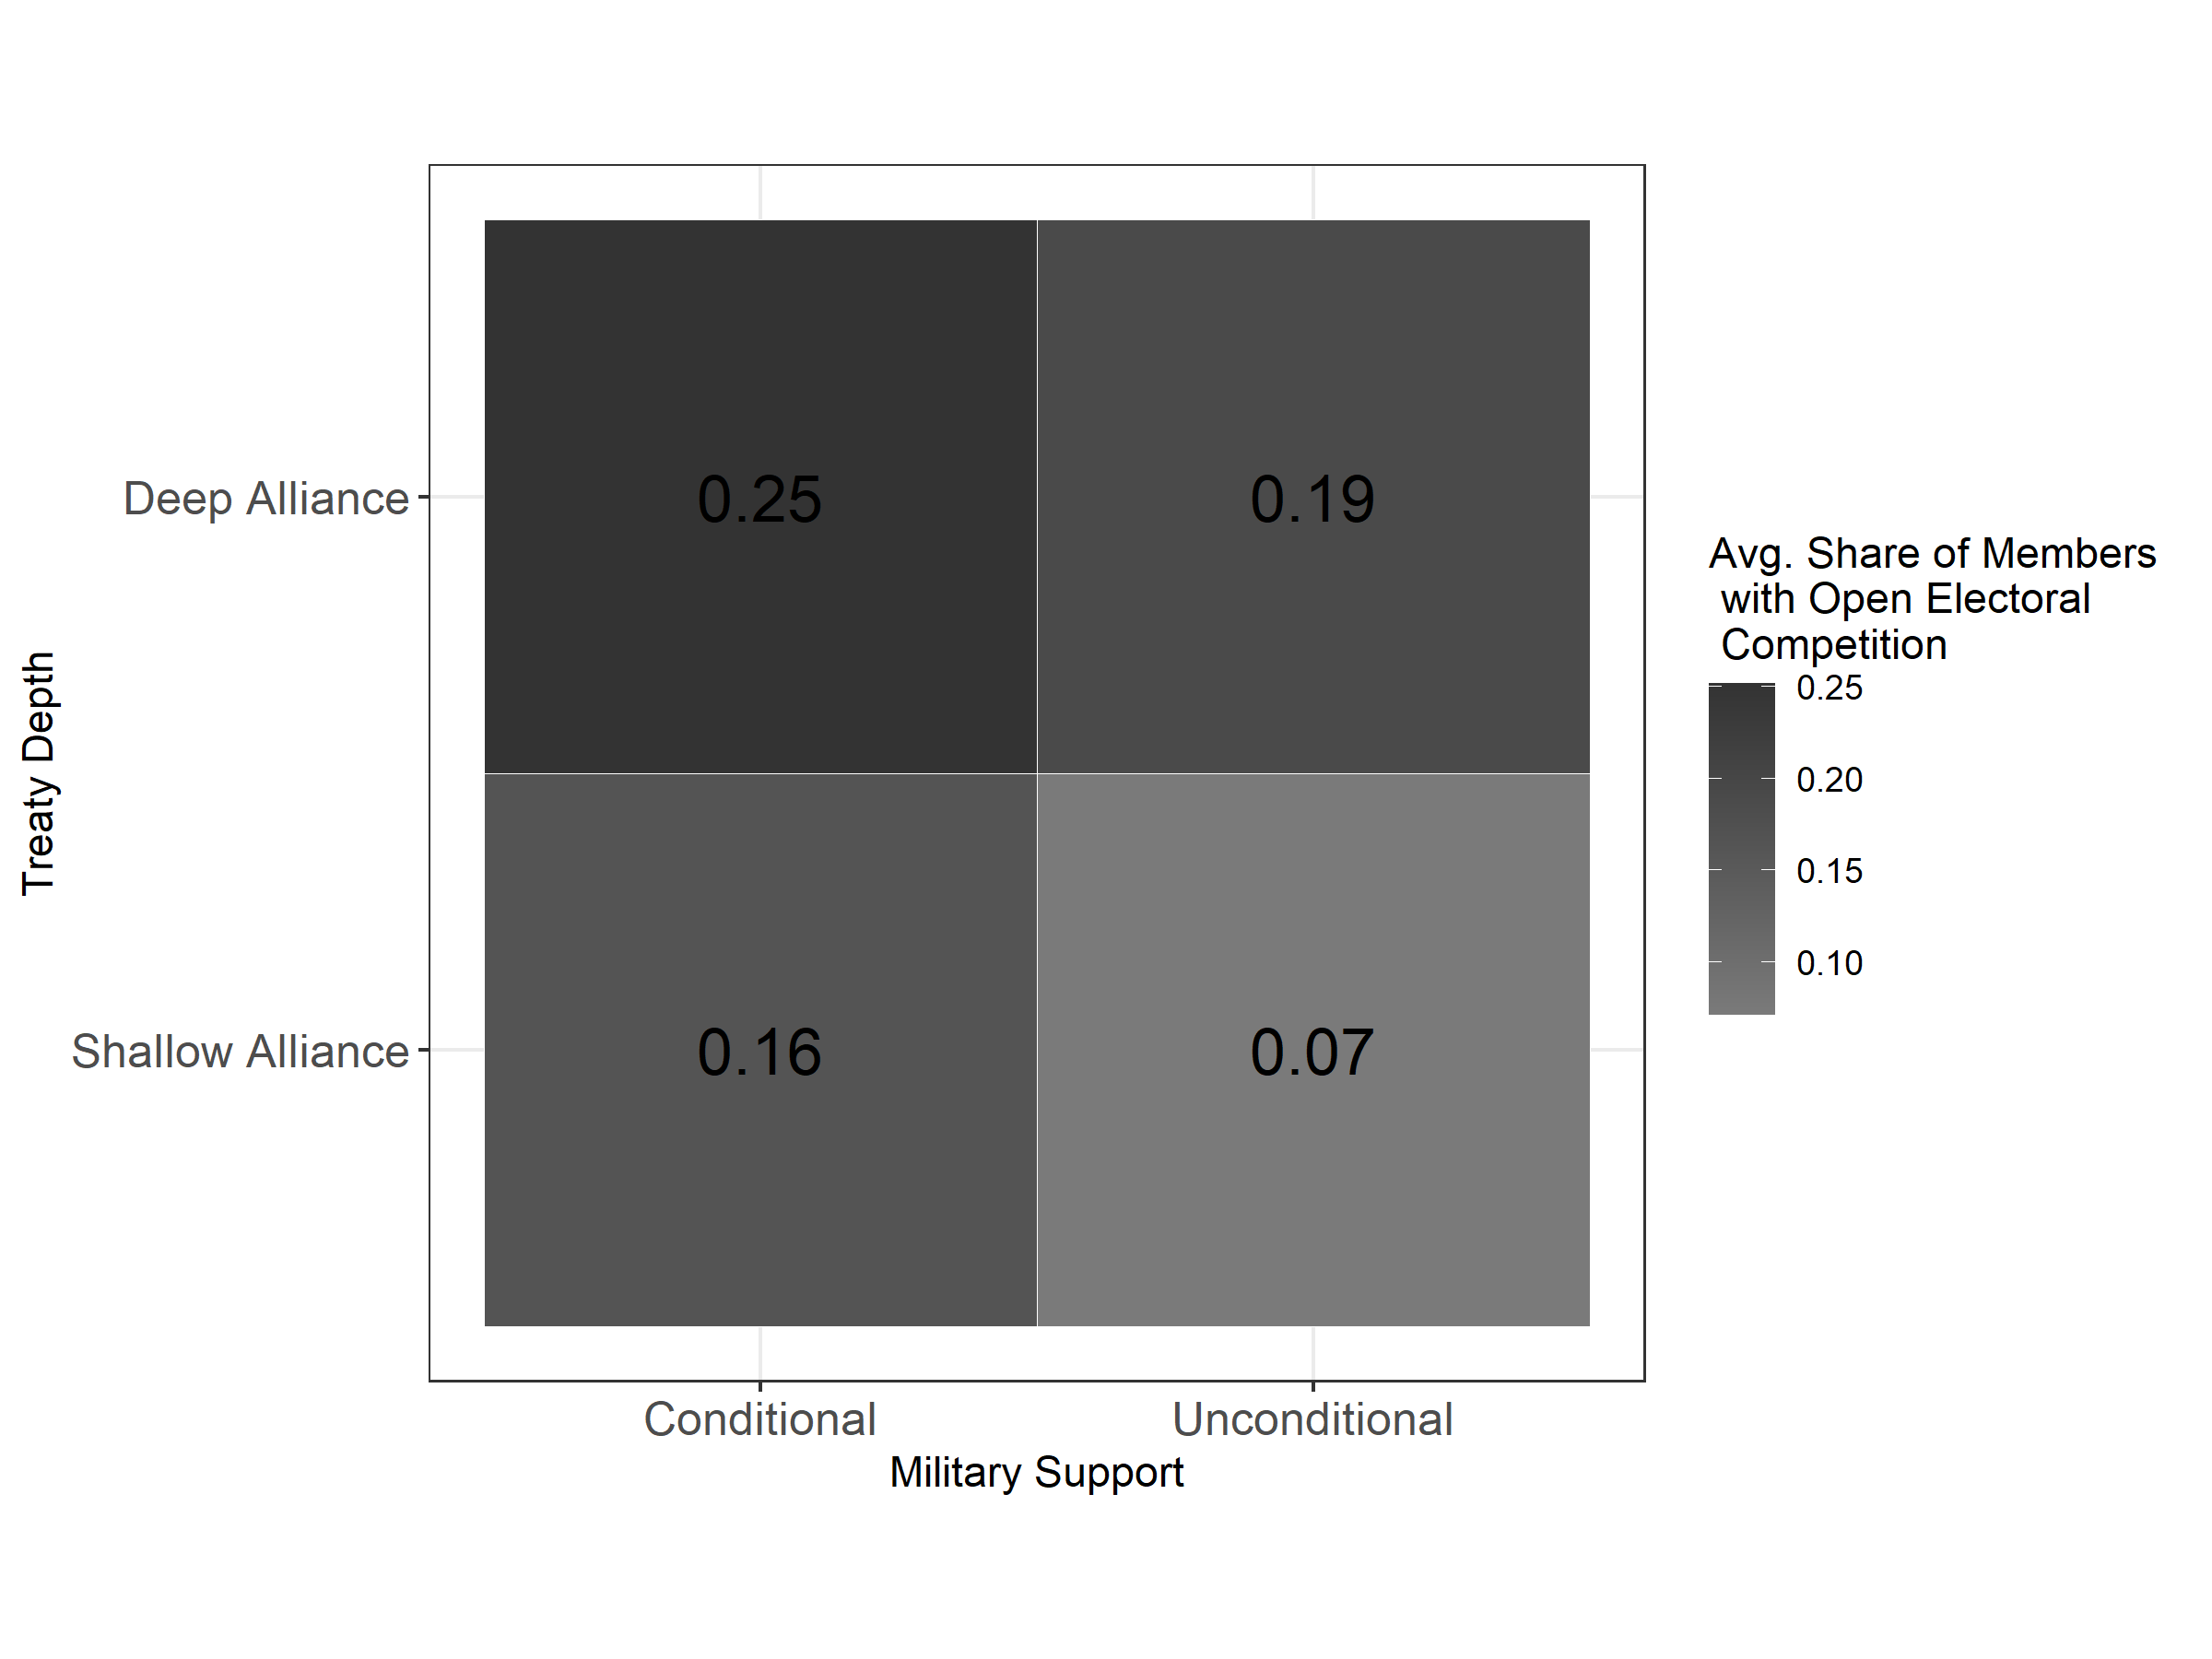
\includegraphics[width=.95\textwidth]{democ-prop-combo.png}  
\caption{Average proportion of democratic members in four groups of alliances. Alliances are grouped based on treaty depth and unconditional military support.}
\label{fig:democ-prop-combo}
\end{figure}


In \autoref{tab:separate-models-prop}, I summarize the results of separate models of unconditional military support.
There is substantial uncertainty in the democratic proportion coefficient for both outcomes. 
These weaker than expected results may reflect differences in influence, or the competing effects of democratic institutions I identified in the paper. 


\begin{table}[!htbp] \centering 
  \caption{} 
  \label{tab:separate-models-prop} 
\begin{tabular}{@{\extracolsep{5pt}}lcc} 
\\[-1.8ex]\hline 
\hline \\[-1.8ex] 
 & \multicolumn{2}{c}{\textit{Dependent variable:}} \\ 
\cline{2-3} 
\\[-1.8ex] & Latent Depth (rescaled) & Unconditional Military Support \\ 
\\[-1.8ex] & \textit{beta} & \textit{probit} \\ 
\\[-1.8ex] & (1) & (2)\\ 
\hline \\[-1.8ex] 
 Proportion of Democracies & 0.125 & $-$0.516 \\ 
  & ($-$0.334, 0.583) & ($-$1.176, 0.145) \\ 
  Foreign Policy Concessions & $-$0.092 & 0.006 \\ 
  & ($-$0.246, 0.061) & ($-$0.214, 0.227) \\ 
  Number of Members & 0.024$^{}$ & $-$0.031 \\ 
  & ($-$0.002, 0.050) & ($-$0.077, 0.015) \\ 
  Wartime Alliance & $-$0.275 & $-$0.980$^{}$ \\ 
  & ($-$0.624, 0.074) & ($-$1.597, $-$0.363) \\ 
  Asymmetric Obligations & 0.283$^{}$ & 0.038 \\ 
  & ($-$0.053, 0.619) & ($-$0.456, 0.532) \\ 
  Asymmetric Capability & 0.346 & 0.600 \\ 
  & ($-$0.123, 0.815) & ($-$0.269, 1.468) \\ 
  Non-Major Only & 0.253 & 1.093$^{}$ \\ 
  & ($-$0.254, 0.760) & (0.209, 1.977) \\ 
  Average Threat & 1.101$^{}$ & 1.645$^{}$ \\ 
  & (0.238, 1.965) & (0.328, 2.961) \\ 
  Foreign Policy Disagreement & 0.117 & 0.384 \\ 
  & ($-$0.339, 0.573) & ($-$0.312, 1.079) \\ 
  Start Year & 0.004$^{}$ & 0.015$^{}$ \\ 
  & (0.001, 0.008) & (0.010, 0.021) \\ 
  Constant & $-$9.468$^{}$ & $-$31.466$^{}$ \\ 
  & ($-$16.269, $-$2.668) & ($-$42.952, $-$19.979) \\ 
 \hline \\[-1.8ex] 
Observations & 277 & 277 \\ 
Log Likelihood & 52.250 & $-$132.053 \\ 
\hline 
\hline \\[-1.8ex] 
\textit{Note:}  & \multicolumn{2}{r}{95\% Confidence Intervals in Parentheses.} \\ 
\end{tabular} 
\end{table} 



The democratic proportion coefficient estimates are sensitive to correlated errors in the depth and unconditional military support models, however. 
Results from a generalized joint regression model of treaty depth and unconditional military support match the findings in the paper, as \autoref{fig:results-prop} shows. 
There is a no substantive association between the proportion of democracies in an alliance and the probability of unconditional military support. 
Alliances between democracies have higher treaty depth, however. 
In the bivariate model find little evidence that alliance with more democracies are more likely undertake conditional obligations, but I do find a positive relationship between democratic alliance membership and treaty depth. 


\begin{figure}
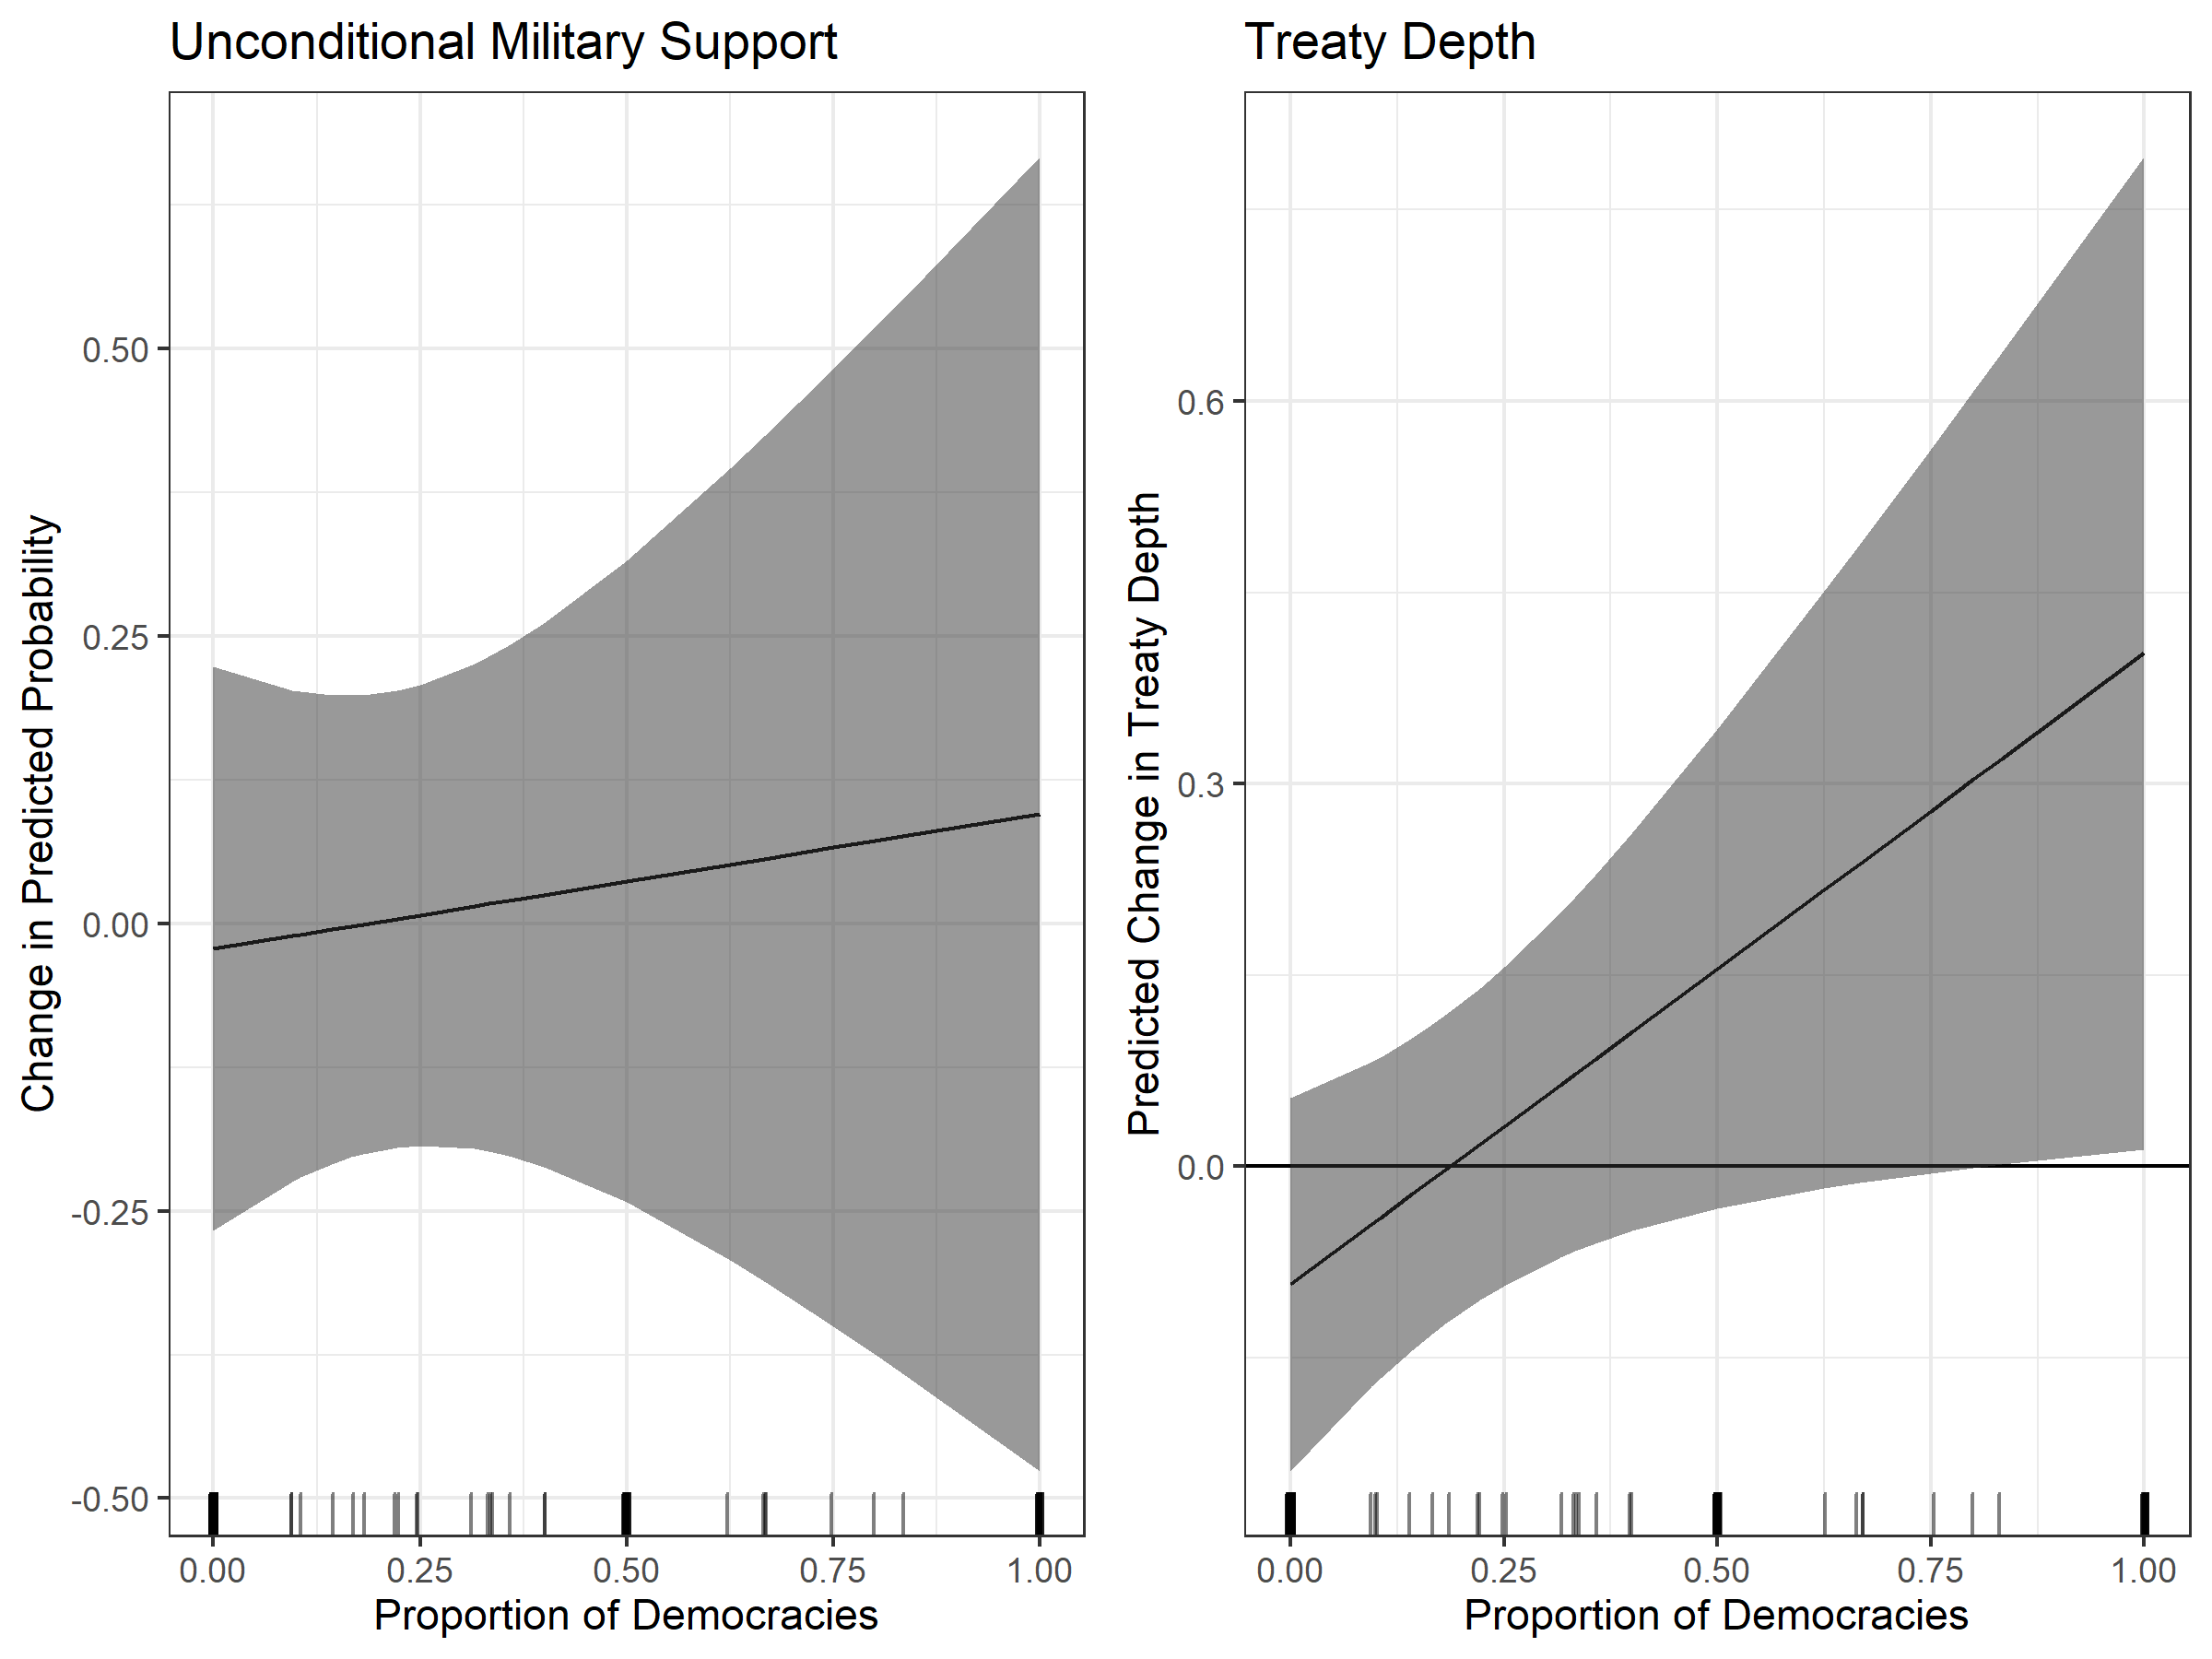
\includegraphics[width=.95\textwidth]{results-prop.png}  
\caption{Predicted probabilities of unconditional military support and predicted changes in treaty depth by the the proportion of democratic alliance members. The line marks predicted values, and the shaded areas encapsulate the standard errors. The rug plot on the x-axis marks observed values of allied democracy. Predictions based on the smoothed terms from the joint generalized regression model.}
\label{fig:results-prop}
\end{figure}



Differences between the joint and separate models of democratic proportion and alliance design are the result of correlations in the error terms of the depth and unconditional support models.  
Kendall's $\tau$ measures the strength of the correlation between the errors, and is a function of a parameter $\theta$ that I modeled in a third GJRM equation.
I used the start year of the alliance to predict differences in $\theta$, which affects correlations in unobservables between depth and unconditional military support. 
\autoref{fig:results-error} plots the smoothed term I used to predict the correlation in the error terms between treaty depth and unconditional military support. 
The predicted values in the top panel of \autoref{fig:results-error} are on the scale of $\theta$. 
In the bottom panel, I plot predicted $\tau$ values against the start year of the alliance. 


\begin{figure}[hbtp]
\centering
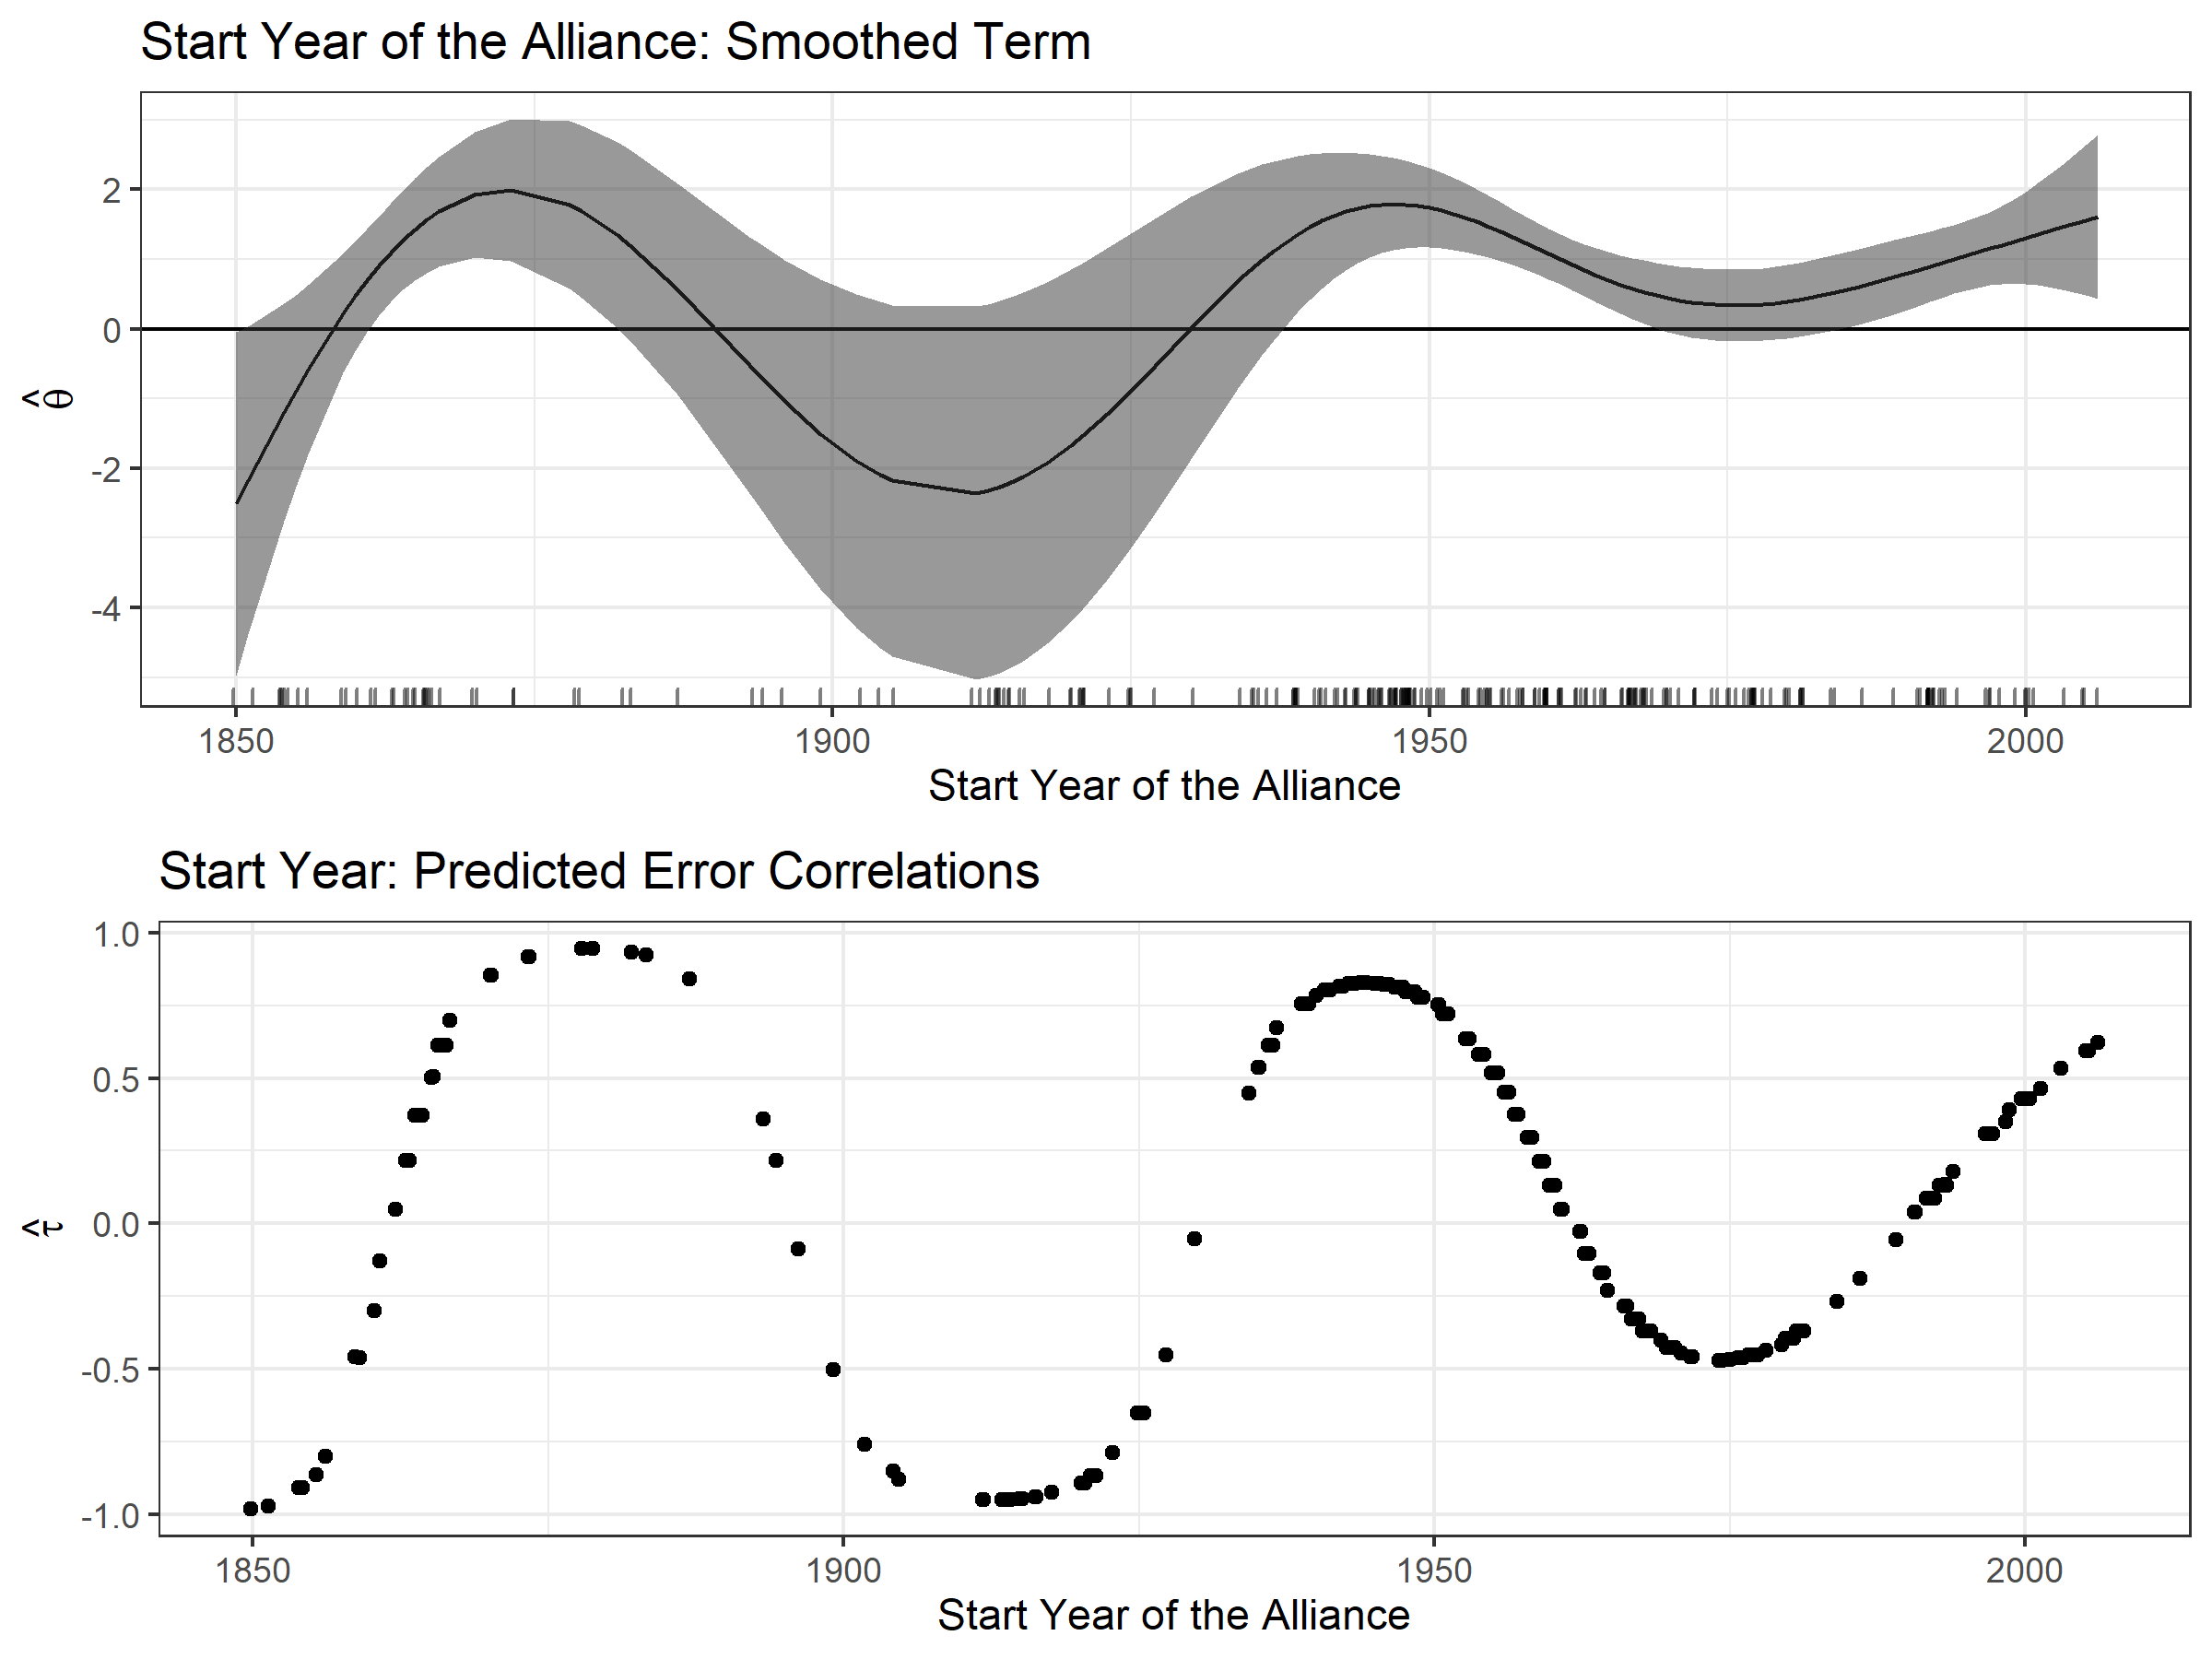
\includegraphics[width=0.95\textwidth]{results-error.png}
\caption{Predicted association between the errors of the unconditional military support and treaty depth equations in a generalized joint regression model by the start year of the alliance. There is limited alliance data before 1850, which dramatically increases uncertainty in the smoothed term. To make the plot more legible I present predictions from after 1850. The rug plot on the x-axis in the top row marks the distribution of alliances. Each point in the bottom row is an estimated $\tau$, one for each of the 277 observations.}
\label{fig:results-error}
\end{figure}


As \autoref{fig:results-error} shows, the association between the errors varies heavily by year. 
Most error correlations are positive between 1850 and 1900, before turning more negative between 1900 and 1950. 
During World War II depth and unconditional military support errors are positively associated. 
In general, the magnitude and direction of estimated correlation between depth and unconditional military support in unobserved factors $\tau$ changes dramatically over time.  


Again, correlations between unobserved factors are responsible for differences in results between the joint model and the separate models. 
This same pattern the error correlations is present in the bivariate GJRM models I report in the paper, but it is less consequential for estimates with the Polity score of the most capable member. 
As a result, the bivariate models are a crucial robustness check. 


\section{Other Measures of Treaty Depth}


To facilitate inferences across a wide range of models with the beta regression, results in the paper are based on rescaled mean latent treaty depth, which ranges between 0 and 1. 
I make similar inferences about treaty depth and the Polity score of the most capable alliance member when I estimate regression models of treaty depth without this transformation, however. 
\autoref{tab:depth-alt-models} summarizes these results. 

\begin{table}[!htbp] 
\centering 
  \caption{Regression models of alliance treaty depth without any transformation. Model 1 uses an OLS estimator, while Models 2 and 3 are robust regressions with Tukey's Biweight function. Model 4 is a binomial model of whether an alliance has median treaty depth or higher. All four models find a positive association between the Polity score of the most capable alliance member and treaty depth.} 
  \label{tab:depth-alt-models} 
\begin{adjustbox}{width= .95\textwidth, center}
\begin{tabular}{@{\extracolsep{5pt}}lcccc} 
\\[-1.8ex]\hline 
\hline \\[-1.8ex] 
 & \multicolumn{4}{c}{\textit{Dependent variable:}} \\ 
\cline{2-5} 
\\[-1.8ex] & \multicolumn{3}{c}{Latent Depth} & Deep Alliance Dummy \\ 
\\[-1.8ex] & \textit{OLS} & \multicolumn{2}{c}{\textit{Robust Reg.}} & \textit{Probit} \\ 
\\[-1.8ex] & (1) & (2) & (3) & (4)\\ 
\hline \\[-1.8ex] 
 Alliance Leader Polity & 0.020$^{}$ & 0.019$^{}$ & 0.028$^{}$ & 0.030$^{}$ \\ 
  & (0.004, 0.035) & (0.003, 0.035) & (0.010, 0.046) & (0.004, 0.056) \\ 
  Foreign Policy Concessions & $-$0.043 & $-$0.043 & $-$0.104 & 0.006 \\ 
  & ($-$0.157, 0.070) & ($-$0.159, 0.073) & ($-$0.239, 0.030) & ($-$0.188, 0.199) \\ 
  Number of Members & 0.015 & 0.017 & 0.017 & 0.033$^{}$ \\ 
  & ($-$0.005, 0.036) & ($-$0.003, 0.038) & ($-$0.004, 0.037) & ($-$0.005, 0.071) \\ 
  Wartime Alliance & $-$0.253$^{}$ & $-$0.240$^{}$ & 0.040 & $-$0.429$^{}$ \\ 
  & ($-$0.511, 0.005) & ($-$0.505, 0.024) & ($-$0.306, 0.386) & ($-$0.877, 0.019) \\ 
  Asymmetric Obligations & 0.101 & 0.126 & 0.293$^{}$ & 0.339 \\ 
  & ($-$0.155, 0.356) & ($-$0.136, 0.388) & ($-$0.040, 0.625) & ($-$0.089, 0.767) \\ 
  Asymmetric Capability & 0.302$^{}$ & 0.283 & 0.212 & 0.671$^{}$ \\ 
  & ($-$0.043, 0.646) & ($-$0.070, 0.636) & ($-$0.499, 0.924) & (0.069, 1.273) \\ 
  Non-Major Only & 0.229 & 0.230 & 0.072 & 0.675$^{}$ \\ 
  & ($-$0.143, 0.601) & ($-$0.151, 0.611) & ($-$0.639, 0.783) & (0.029, 1.321) \\ 
  Average Threat & 0.963$^{}$ & 0.965$^{}$ & 1.424$^{}$ & 1.881$^{}$ \\ 
  & (0.317, 1.608) & (0.303, 1.626) & (0.650, 2.198) & (0.748, 3.014) \\ 
  Foreign Policy Disagreement & 0.180 & 0.161 & 0.333 & 0.279 \\ 
  & ($-$0.158, 0.517) & ($-$0.185, 0.507) & ($-$0.104, 0.770) & ($-$0.294, 0.853) \\ 
  Start Year & 0.003$^{}$ & 0.003$^{}$ & 0.021$^{}$ & 0.001 \\ 
  & (0.0003, 0.005) & (0.00001, 0.005) & (0.014, 0.027) & ($-$0.003, 0.006) \\ 
  Constant & $-$6.226$^{}$ & $-$5.789$^{}$ & $-$41.431$^{}$ & $-$4.431 \\ 
  & ($-$11.203, $-$1.249) & ($-$10.890, $-$0.688) & ($-$53.699, $-$29.162) & ($-$12.869, 4.006) \\ 
 \hline \\[-1.8ex] 
Observations & 279 & 279 & 203 & 279 \\ 
\hline 
\hline \\[-1.8ex] 
\textit{Note:}  & \multicolumn{4}{r}{95\% Confidence Intervals in Parentheses.} \\ 
\end{tabular}
\end{adjustbox} 
\end{table} 


In \autoref{tab:depth-alt-models}, I include inferences from OLS, a robust regression estimator, and a probit GLM. 
The robust regression re-weights observations to correct for non-normal residuals and influential observations that might bias inferences from the OLS estimator. 
Model 3 is a robust regression of alliances after 1919, which is the same timeframe as \citep{Mattes2012}. 
In the probit model, the outcome is dummy variable that I set equal to one if the alliance has higher than the median latent depth. 


In addition to these checks, I examine the association between alliance leader democracy and two measures in existing scholarship with some similarity to treaty depth. 
\citet{LeedsAnac2005} develop an ordinal measure of military institutionalization.
\citet{BensonClinton2016} use a latent variable model to model treaty depth, but their measure of treaty depth reflects a different concept; the overall costliness of the alliance obligations. 
While my measure is a better fit for my purposes in this paper, I find that the Polity score of the alliance leader is also positively correlated with these two variables. 


Alliance leader democracy is positively correlated with the Leeds and Anac measure of military institutionalization in separate and joint models, but the correlation in joint models is weaker.
This measure is a useful first step towards measuring defense cooperation, but it understates the amount of variation in treaty depth. 
\citet{LeedsAnac2005} argue that commitments of an integrated military command, common defense policy, or any basing rights generate high military institutionalization. 
Official contact between military officials, formal organizations, providing training or technology, subordination of forces, or specific contributions reflect moderate institutionalization. 
If at least one of the relvant factors is present, Leeds and Anac assign alliance the highest corresponding level of institutionalization. 
This approach assumes that alliances with multiple sources of depth as just as deep/institutionalized as alliances with one source, which understates the amount of variation in alliance treaty depth.


\begin{figure}[htbp]
	\centering
		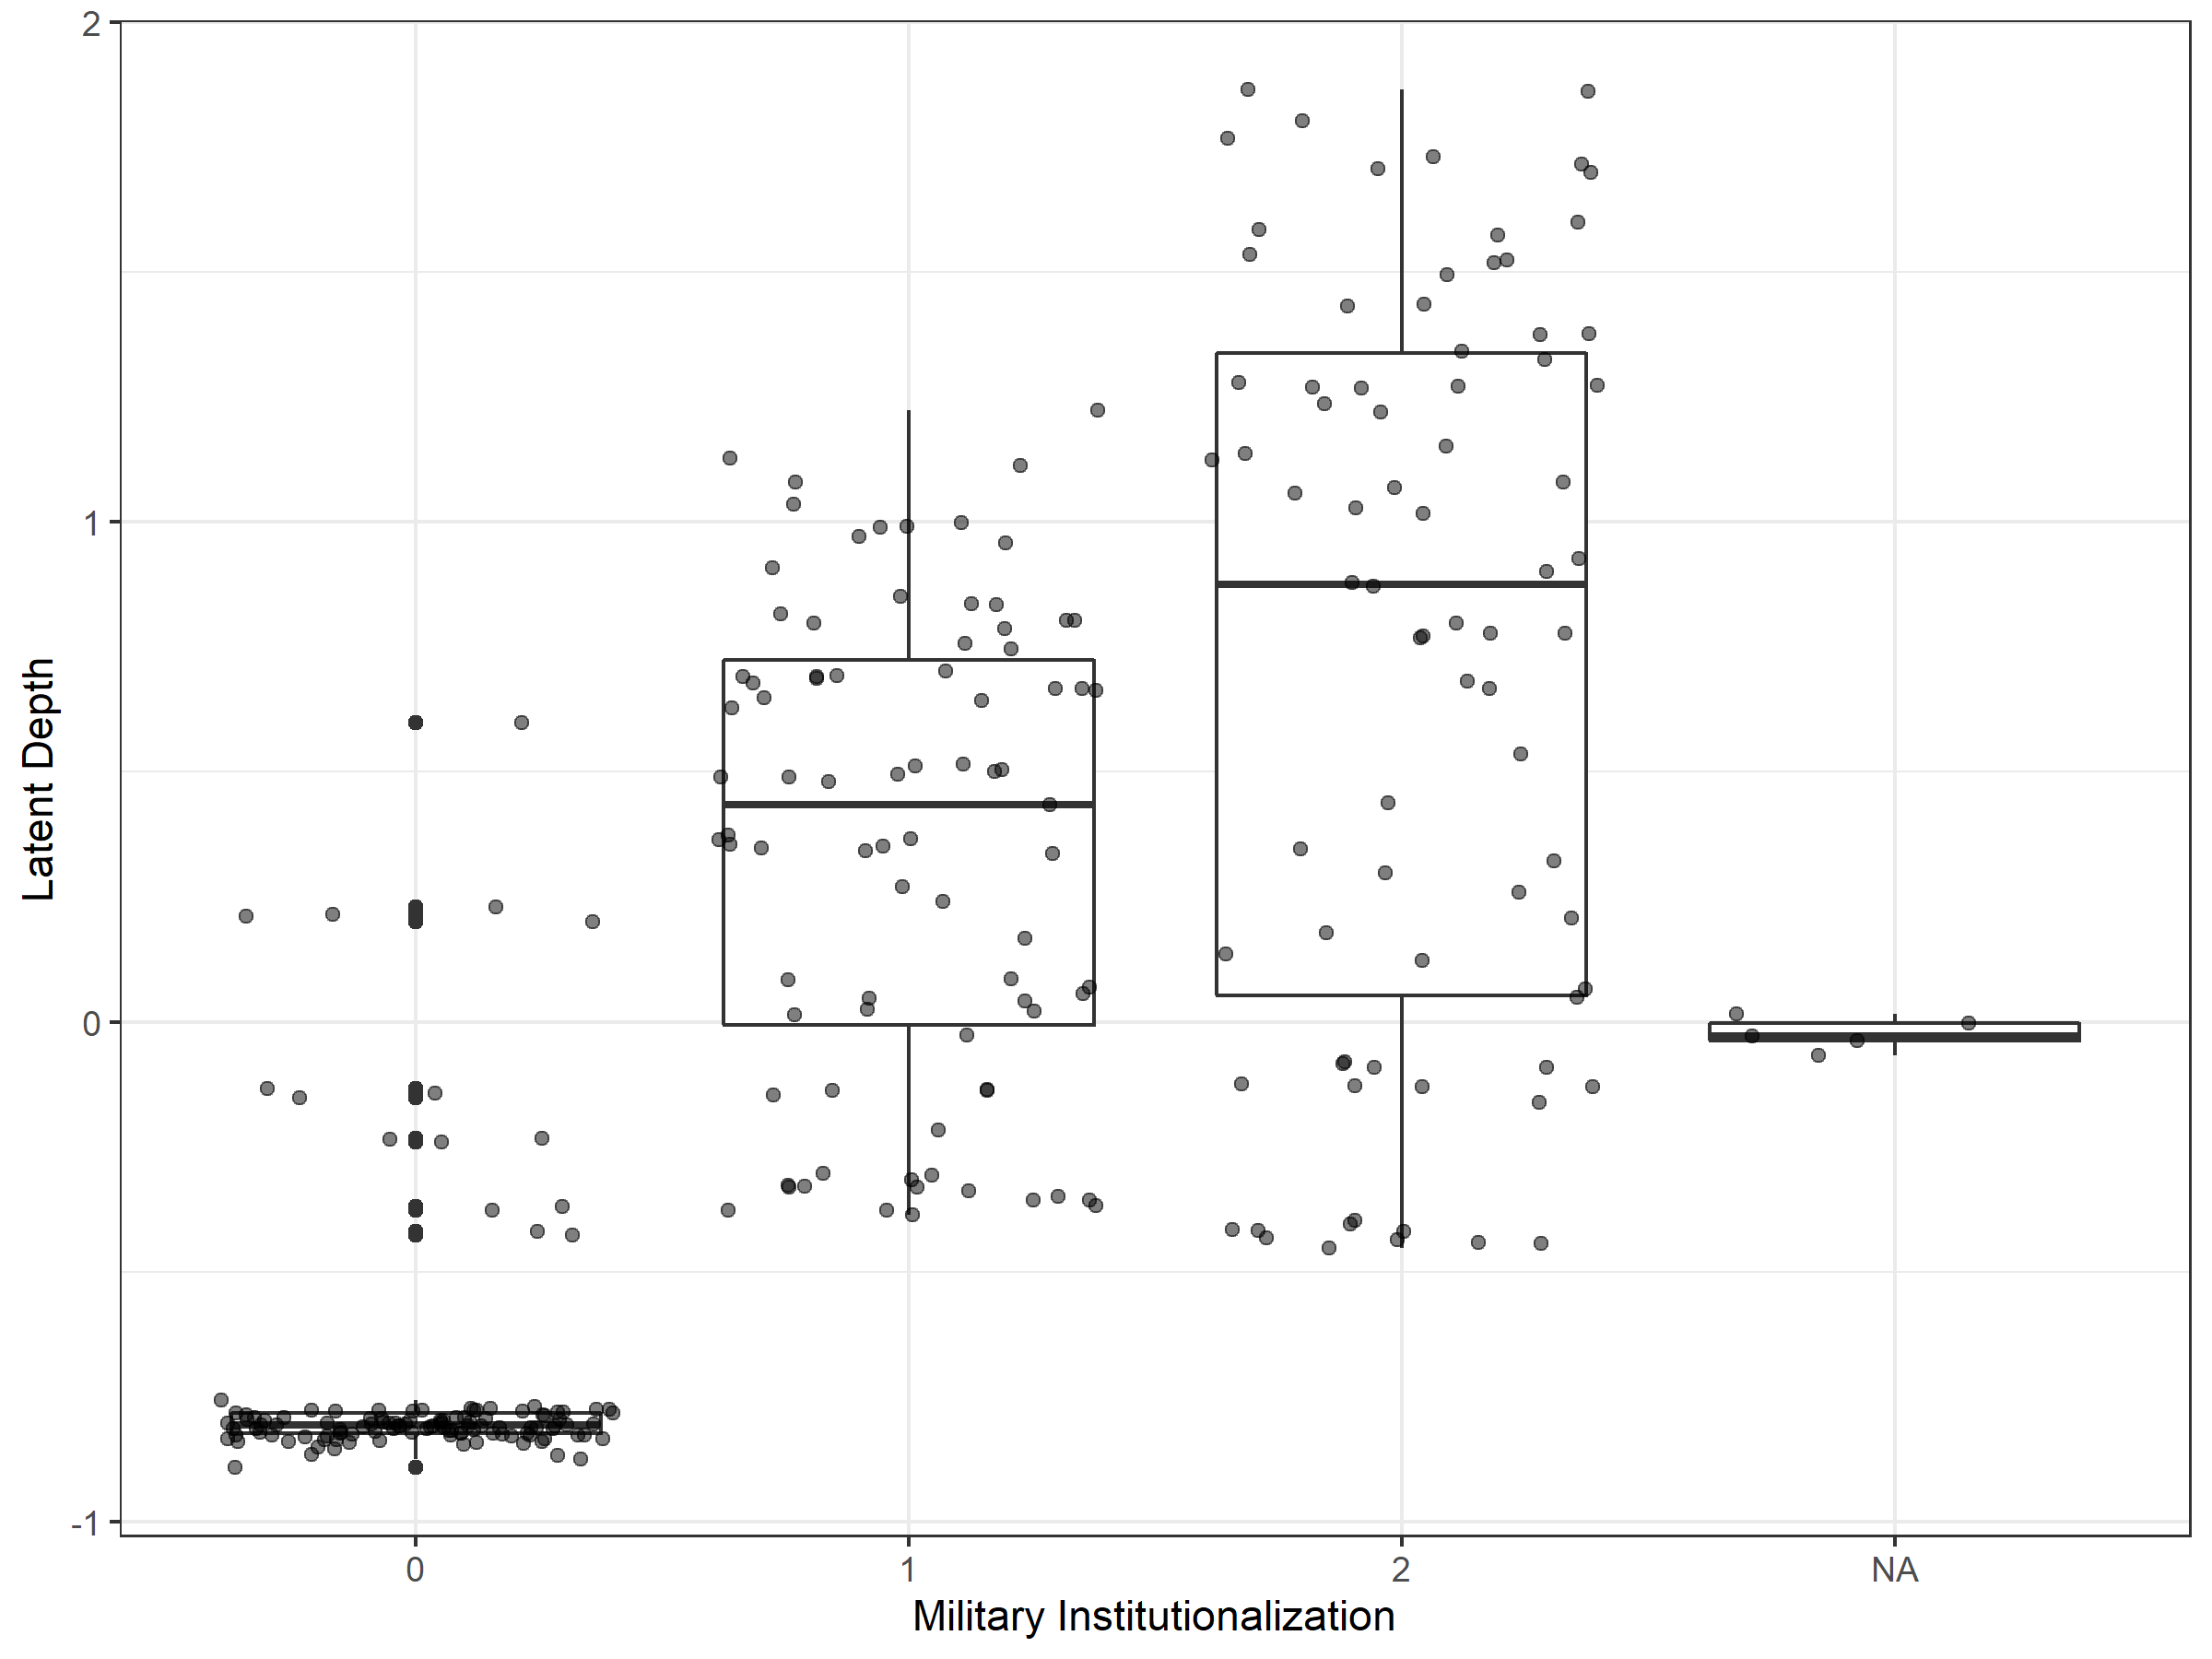
\includegraphics[width=0.95\textwidth]{milinst-comp.png}
	\caption{Scatter plot of latent treaty depth across the values of military institutionalization from \citet{LeedsAnac2005}. The box plots summarize the distribution of latent treaty depth within each category of military institutionalization. Points are jittered within each level of the institutionalization score.}
	\label{fig:milinst-comp}
\end{figure} 

As \autoref{fig:milinst-comp} shows, the ordinal variable is positively correlated with my latent measure, but there is substantial variation in the latent measure within each category. 
The deepest alliances on the latent measure also have the highest military institutionalization score.
There are substantial differences within each category and overlap in the latent scores across the categories, however. 
For example, some alliances that \citet{LeedsAnac2005} assign a moderate institutionalization score have more depth than alliances with high institutionalization scores because these alliance treaties contain multiple sources of depth. 
Within each level of the military institutionalization factor, there is a substantial variation in treaty depth. 


The Benson and Clinton measure is harder to compare, because it addresses a different concept, covers fewer alliances and has more outliers that may impact inferences.
Benson and Clinton's emphasis on the general costliness of the alliance means they include measures of issue linkages and secrecy, which are distinct from defense cooperation. 
Their measure is also based on version 3 of the ATOP data, so it has more limited temporal coverage. 
Last, their latent variable model makes a series of distributional assumptions that may affect the estimated distribution of the latent variable. 
My latent variable is based on a semiparametric model that accounts for dependencies between the factors and latent variables, so the distribution of the latent variable may be more accurate \citep{Murrayetal2013}.
Despite these differences, I find a positive association between the Polity score of the most capable alliance member and Benson and Clinton's measure of depth. 


I now discuss the results of analyses with these other dependent variables. 
As in the paper, I start with univariate models, then move the bivariate models. 
First, I fit an ordinal model of military institutionalization. 
Then, I fit a beta regression model with the rescaled values of Benson and Clinton's depth measure. 
\autoref{fig:results-alt-measures-sep} plots the substantive effect of the leading state's Polity score on both outcomes. 
Democratic institutions in the alliance leader increase the probability of high institutionalization and decrease the probability of no institutionalization. 
Alliance leader democracy is also positively associated with Benson and Clinton's measure of depth. 


\begin{figure}
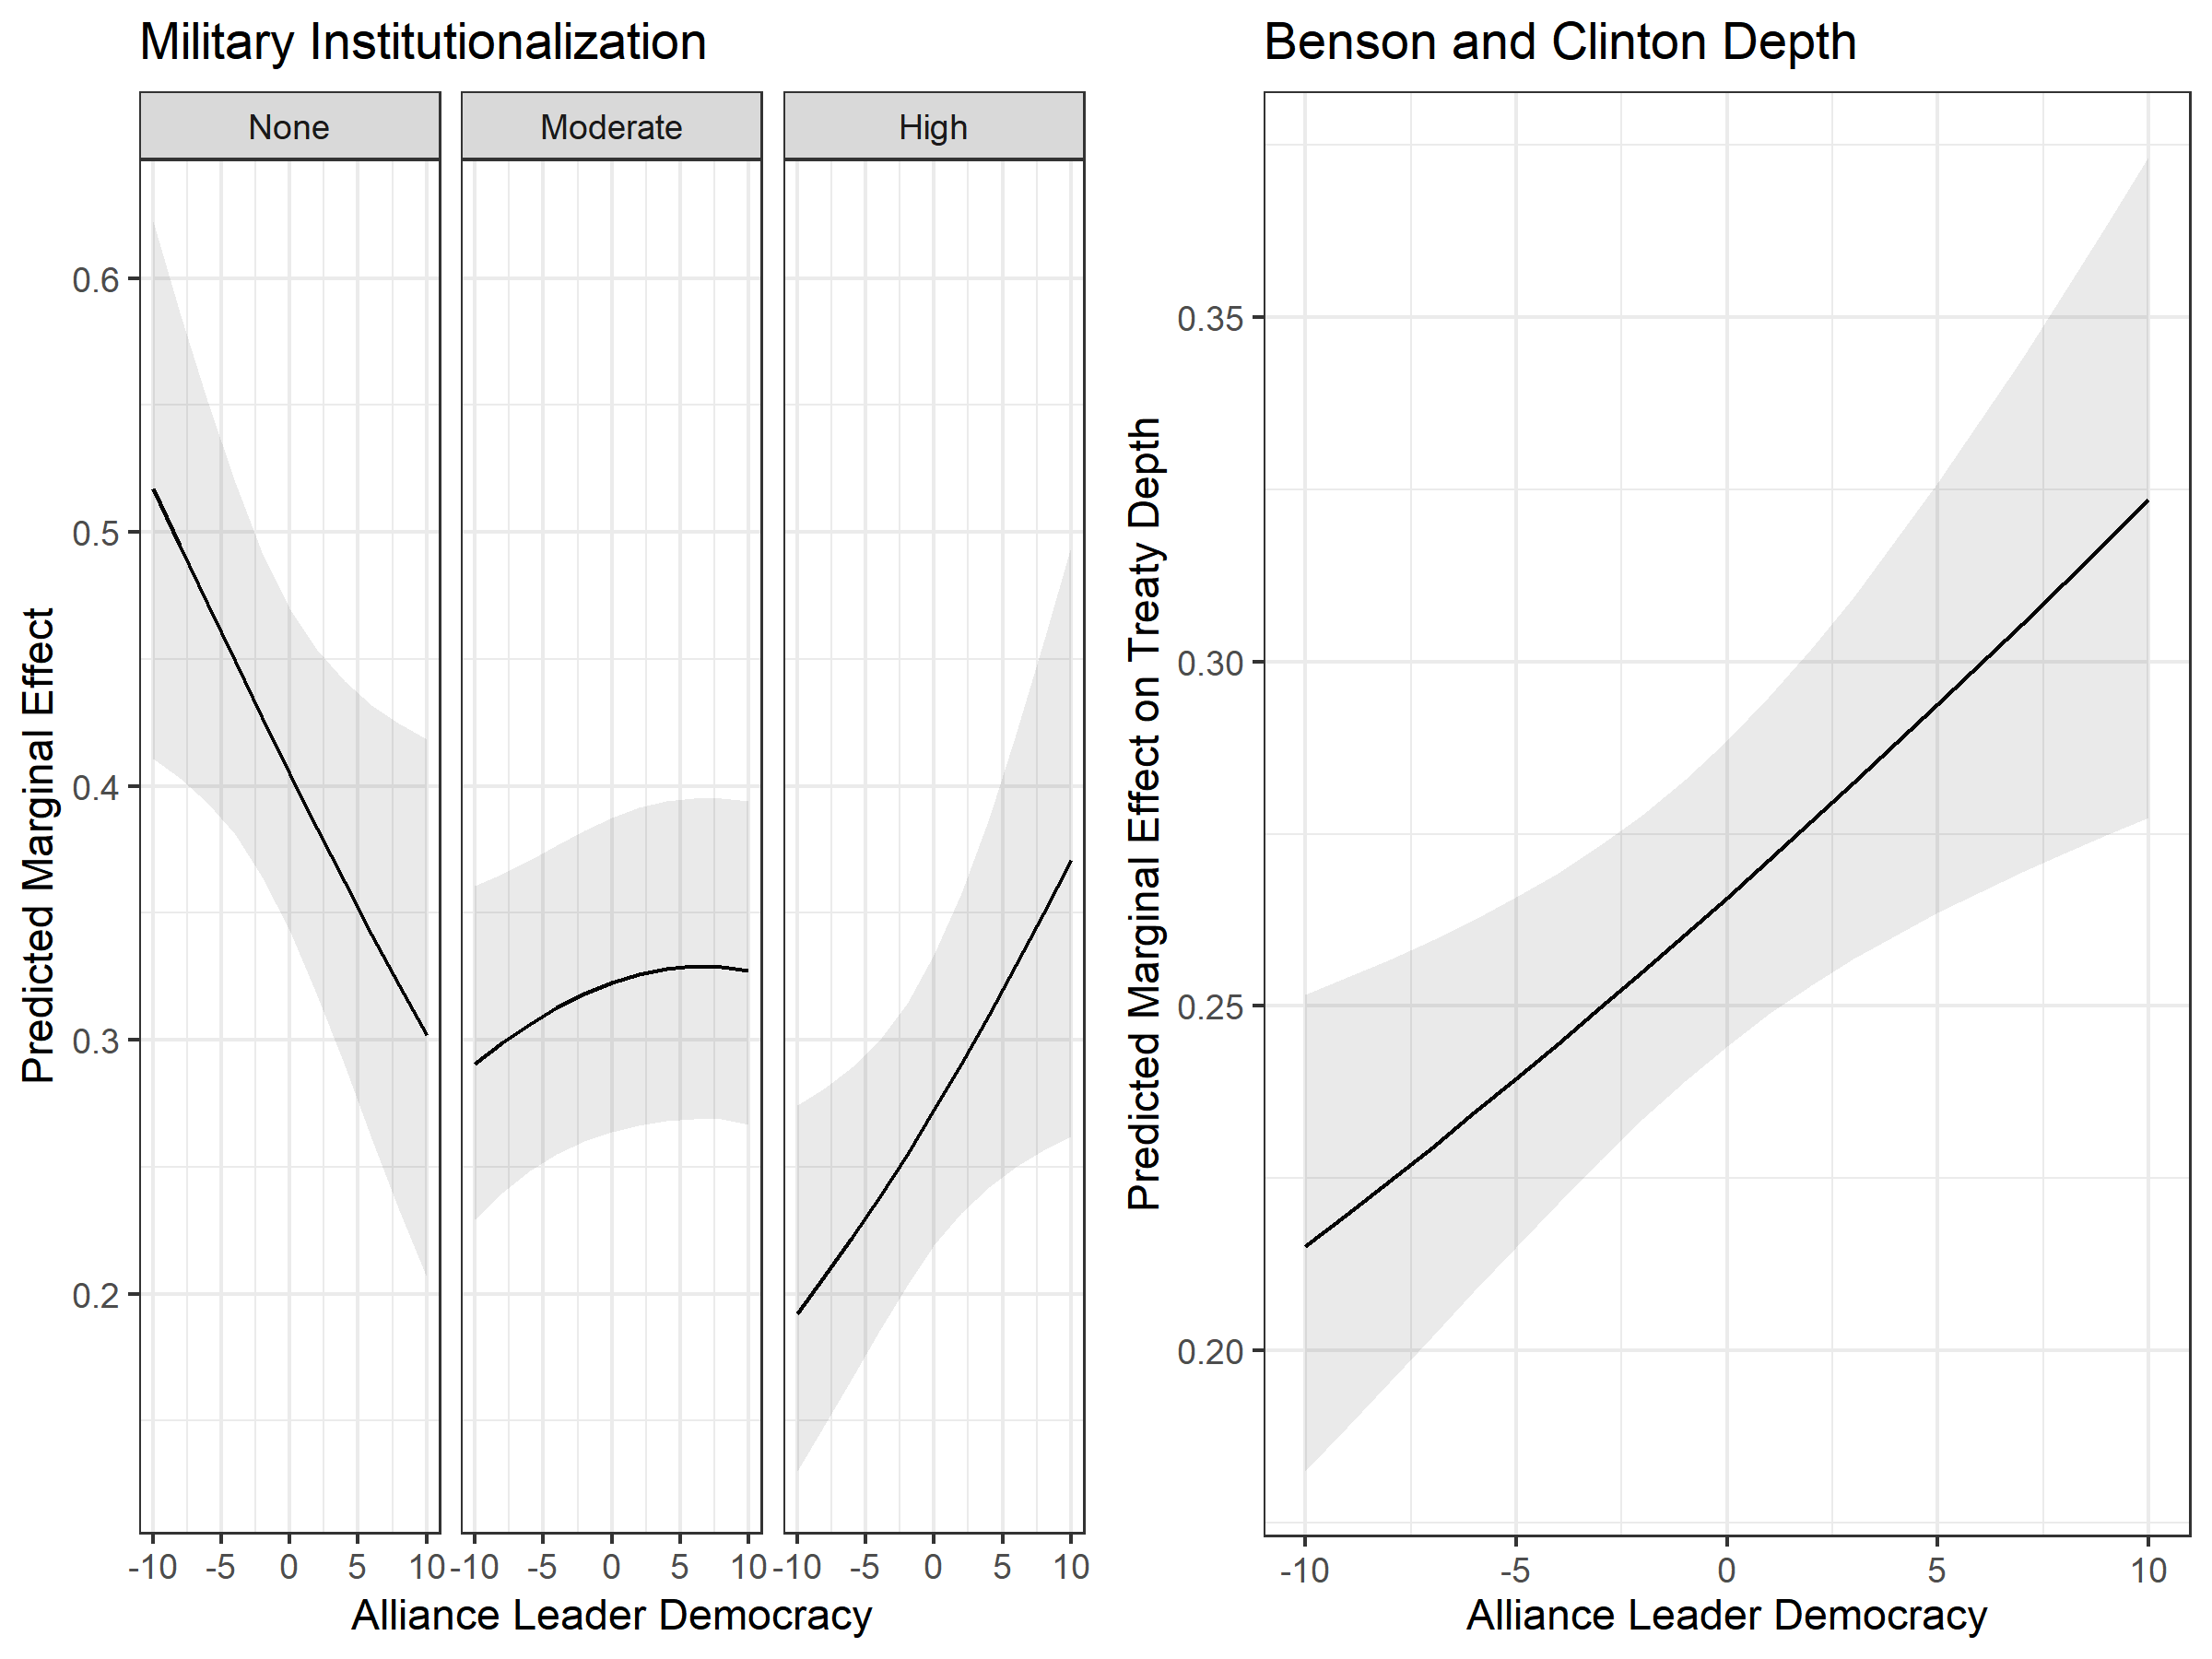
\includegraphics[width=.95\textwidth]{results-alt-measures-sep.png}  
\caption{Predicted changes in treaty depth by the Polity score of the most capable alliance member. The line marks predicted values, and the shaded areas encapsulate the 95\% confidence interval.}
\label{fig:results-alt-measures-sep}
\end{figure}


\autoref{fig:results-alt-measures} plots predictions from the two other depth measures based on bivariate GJRM models. 
For the military institutionalization measure, I could not fit an ordinal model in GJRM. 
Therefore, I created a dummy variable which is equal to one if the alliance had an institutionalization score of 2. 
I then used a probit estimator to model the high military institutionalization dummy. 
The results of this analysis are weaker than expected. 
As the left panel of \autoref{fig:results-alt-measures} shows, although the the probability of high military institutionalization increases with alliance leader democracy, the increase is small. 
This may reflect that the ordinal measure understates variation in alliance treaty depth. 


\begin{figure}
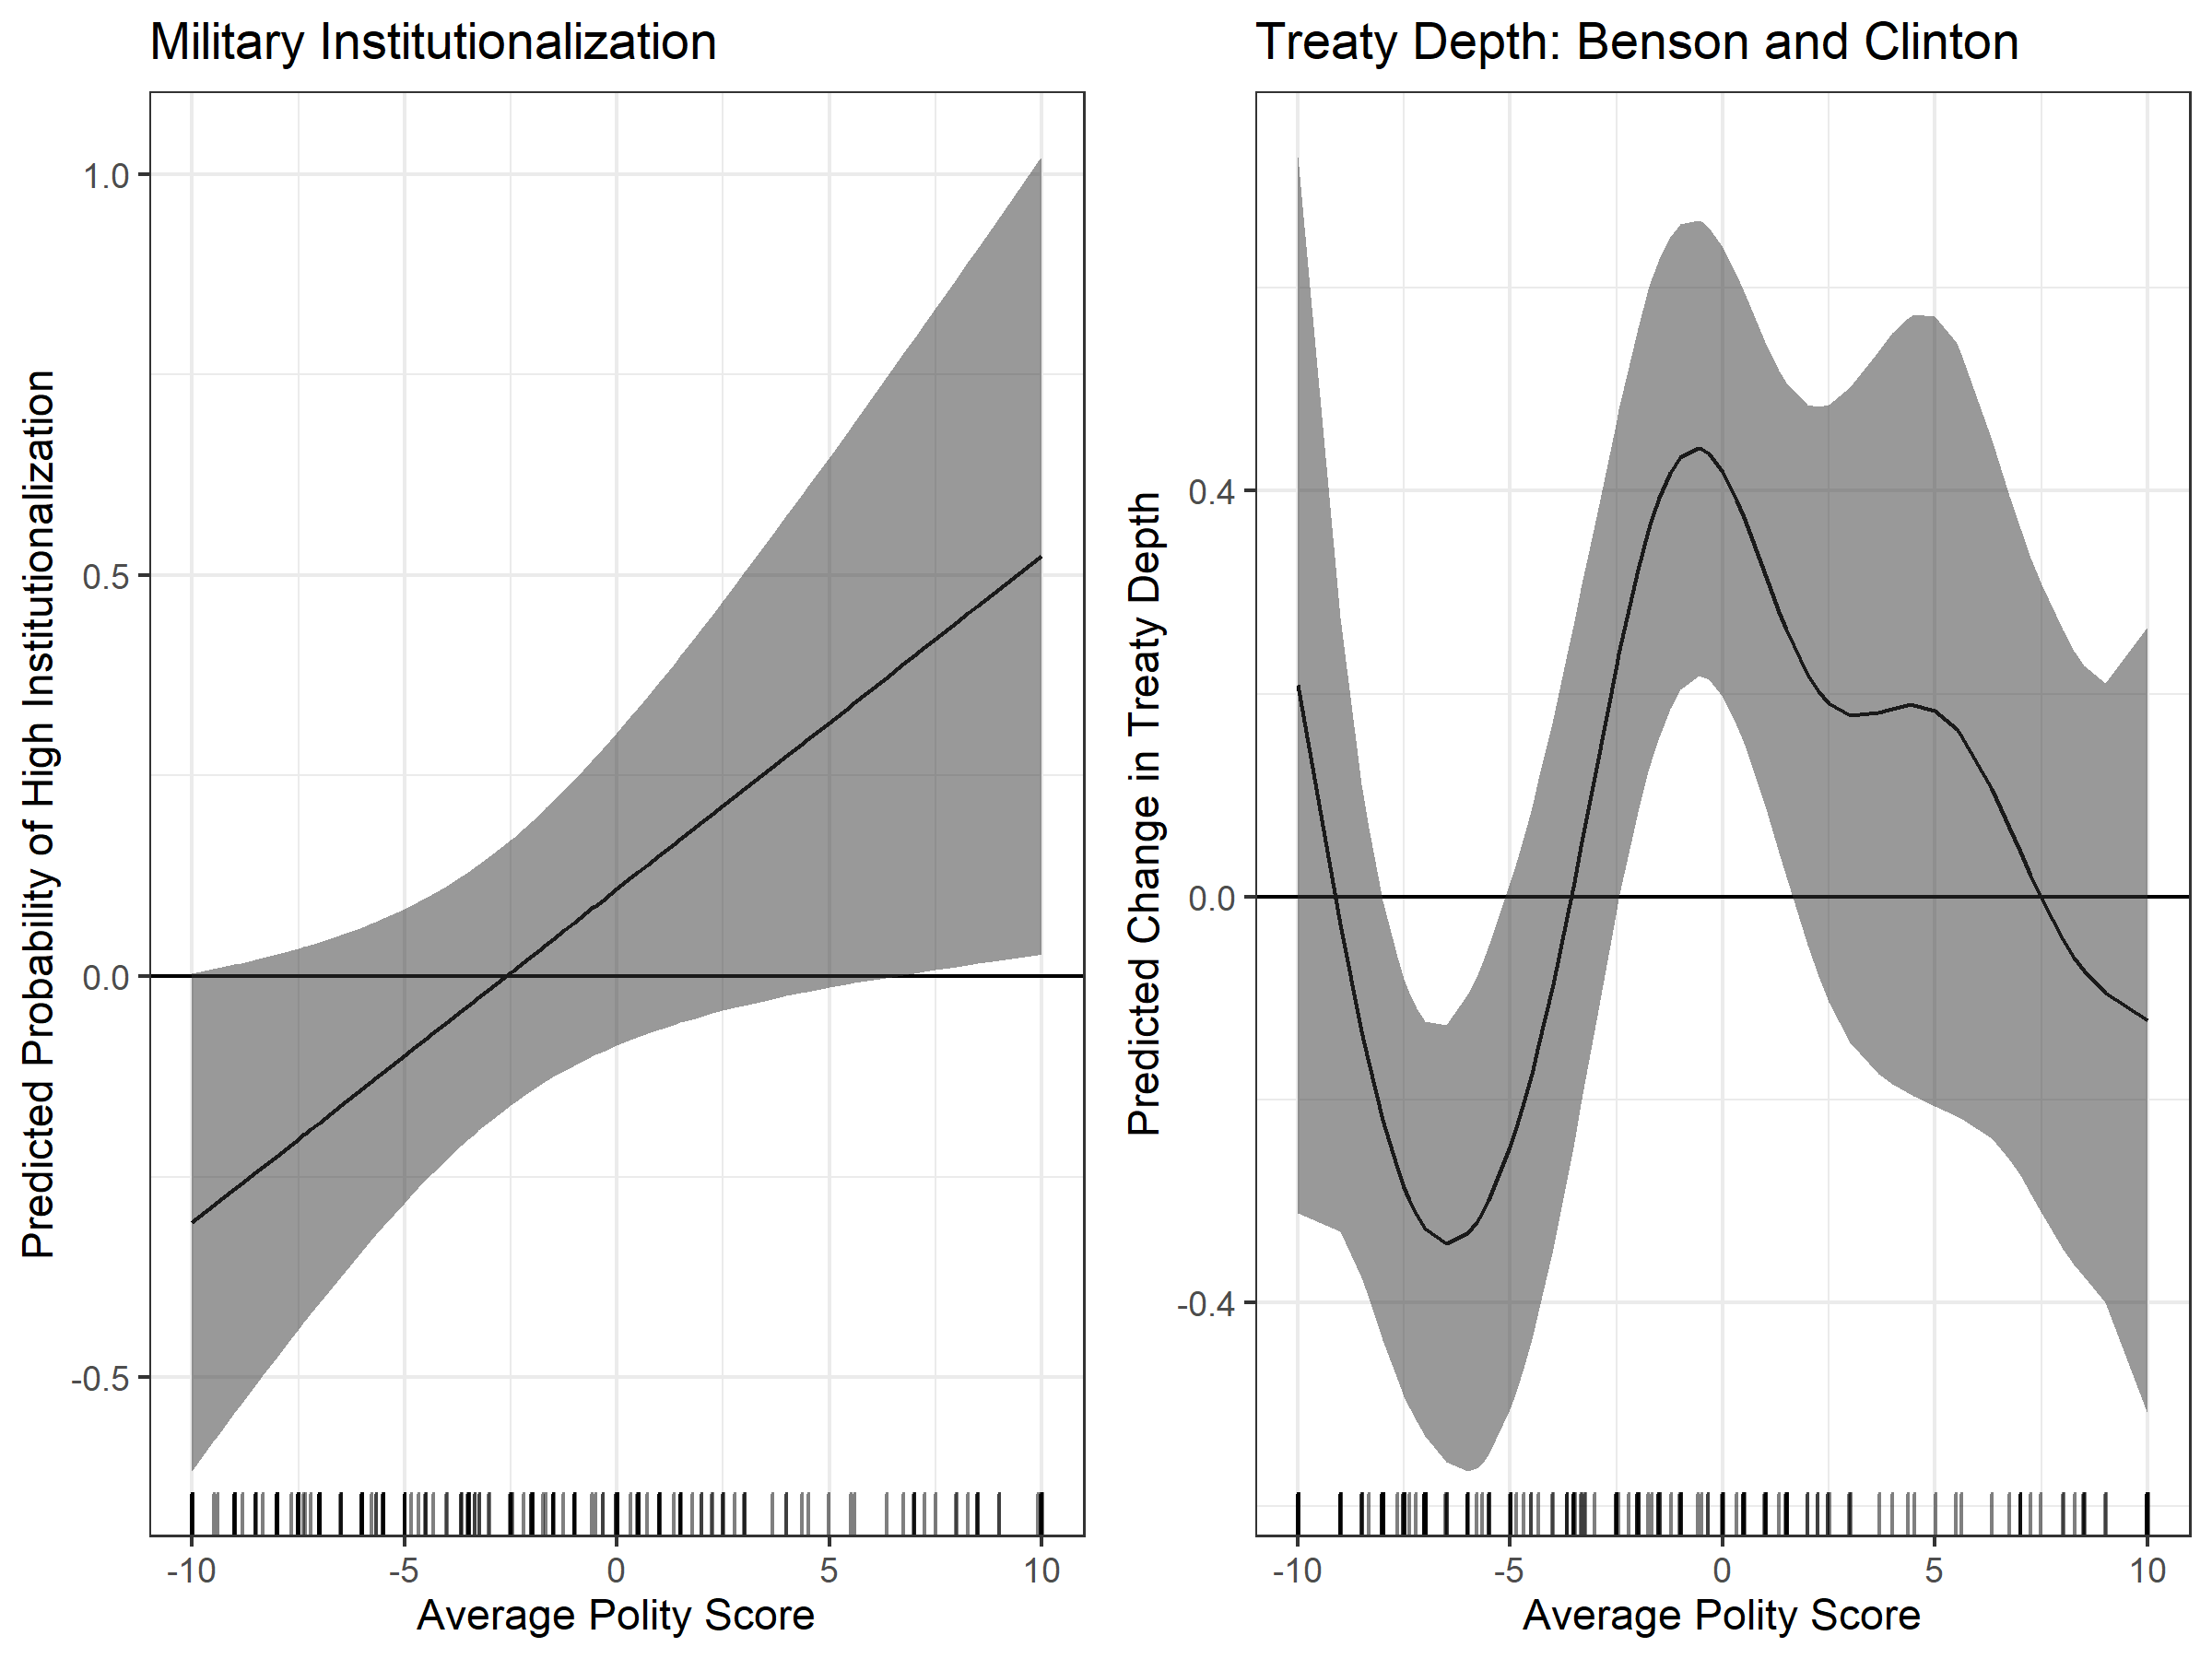
\includegraphics[width=.95\textwidth]{results-alt-measures.png}  
\caption{Predicted probability of military institutionalization and predicted treaty depth as a function of alliance leader democracy. The line marks predicted values, and the error bars summarize the approximate 95\% confidence interval. Predictions based on the smoothed terms from two joint generalized regression models, one for military institutionalization and unconditional support, and another with Benson and Clinton's depth measure and unconditional military support. }
\label{fig:results-alt-measures}
\end{figure}

Findings about the association between treaty depth and Benson and Clinton's also match the treaty depth hypothesis. 
Moving from an autocratic to a democratic alliance leader increases the overall costliness of the alliance obligations. 
I expect that this result is driven by the defense cooperation measures in Benson and Clinton's latent measure. 



\section{Adjusting for Alliance Formation}


Observed alliances are the result of negotiations between potential members. 
Therefore the set of observed alliances is not a random sample \citep{Poast2019a}.
Rather, alliances are groups of states that overcame obstacles to alliance formation.  
In this section, I account for non-random alliance formation using a hurdle model of observed alliances and a stratified random sample of non-allied groups of states. 
This research design produces similar inferences: the Polity score of the most capable alliance member increases treaty depth but has no effect on unconditional military support. 


My research design for this robustness check follows existing procedures for dealing with selection into alliances and treaty design. 
First I followed the suggestions of \citet{Poast2010} for dealing with k-adic data, because some alliances have more than two members. 
First I constructed a random sample of groups of states that could have formed an alliance in each year, but did not \citep{FordhamPoast2014}.
I then took a stratified sample of the non-allied k-ads to include five times as many non-allied observations as alliance observations for each observed value of alliance size. 
For example, there are 215 bilateral alliances, so I included 1075 non-allied bilateral groups. 
There is only one alliance with 34 members, so I include five non-alled k-ads with 34 members. 
Finally, I summarized key characteristics of these non-allied k-ads, including average Polity score, the Polity score of the most capable member, the number of members, mean threat, asymmetric capability, and wartime, and merged non-allied data with the observed alliance data. 


To account for alliance design, I built on the research design of \citet{Chibaetal2015}. 
They used a hurdle model to assess whether after accounting for non-random selection into alliances, democracies were more likely to offer conditional obligations.
Hurdle models have two stages or parts.
A first stage model predicts which observations clear the hurdle to a second stage where the outcome is observed. 
Unlike a sample selection model, the second stage in a hurdle model is logically undefined, which is how alliance treaty design works.\footnote{Hurdle models also do not require an exclusion restriction.} 
Unless states overcome the barriers to alliance formation, treaty content cannot exist. 


Unlike \citet{Chibaetal2015}, I am interested in two aspects of alliance treaty design. 
Therefore, I jointly estimate two hurdle models- one for the depth and the other for unconditional military support. 
To have zero values for the outcome at the hurdle stage, I adjusted the outcomes in these models. 
First, I rescaled latent depth by adding one, which shifted the distribution onto uniformly positive values. 
I then applied a gamma hurdle model to this rescaled depth outcome and used the same covariates as the main model in the manuscript to predict depth. 
For unconditional military support, I replaced the dummy indicator in the manuscript with an ordinal indicator.
This ordinal variable is captures the relative strength of the military support promise in the alliance. 
ATOP alliances can be conditional on four things: adversaries, locations, a particular conflict, the number of opponents, a specific demand or non-provocation in the case of defense treaties. 
The maximum number of observed conditions in an alliance is four, which is the most conditional and limited alliance in the data. 
I therefore invert the number of conditions and assign unconditional alliances a value of four. 
Essentially, the measure then captures the number of circumstances where an alliance could have applied conditions but did not. 
To avoid including zeros in the measure, I add one to it, because promising military support adds some baseline strength to any alliance \citep{Morrow2000}. 
Thus, the final measure of military support commitment strength ranges between 1 and 5 for observed alliances, but is zero for non-alliances. 


In both models, I use average democracy, mean threat, asymmetric capability, wartime, and year varying intercepts to predict whether the group clears the alliance formation hurdle.
In the second stage, I use the democracy of the most capable alliance member, the number of members, mean threat, dummy indicators of asymmetric capability or non-major power only membership, wartime and year varying intercepts to model treaty design. 
I then estimate the two hurdle models simultaneously using the BRMS package for R, which employs STAN for fully Bayesian inference \citep{Buerkner2017}. 
Unlike the GJRM models in the manuscripts, there is no correlation between the residuals of the separate hurdle models. Instead, I connect the two models with a correlated set of year varying intercepts. 
The complexity of this joint hurdle model and limited sample size in the second stage means results should be treated with caution.\footnote{I find similar results with separate hurdle models for depth and conditions on military support. Results on file with the author.} 


Even after accounting for non-random alliance formation with the joint hurdle model, I find similar results to the appendix. 
\autoref{fig:results-joint-hurdle} plots the results of the joint hurdle model. 
As in the sample with only observed alliances, greater democracy among alliance members has no clear relationship with conditionality, but increases treaty depth. 


\begin{figure}
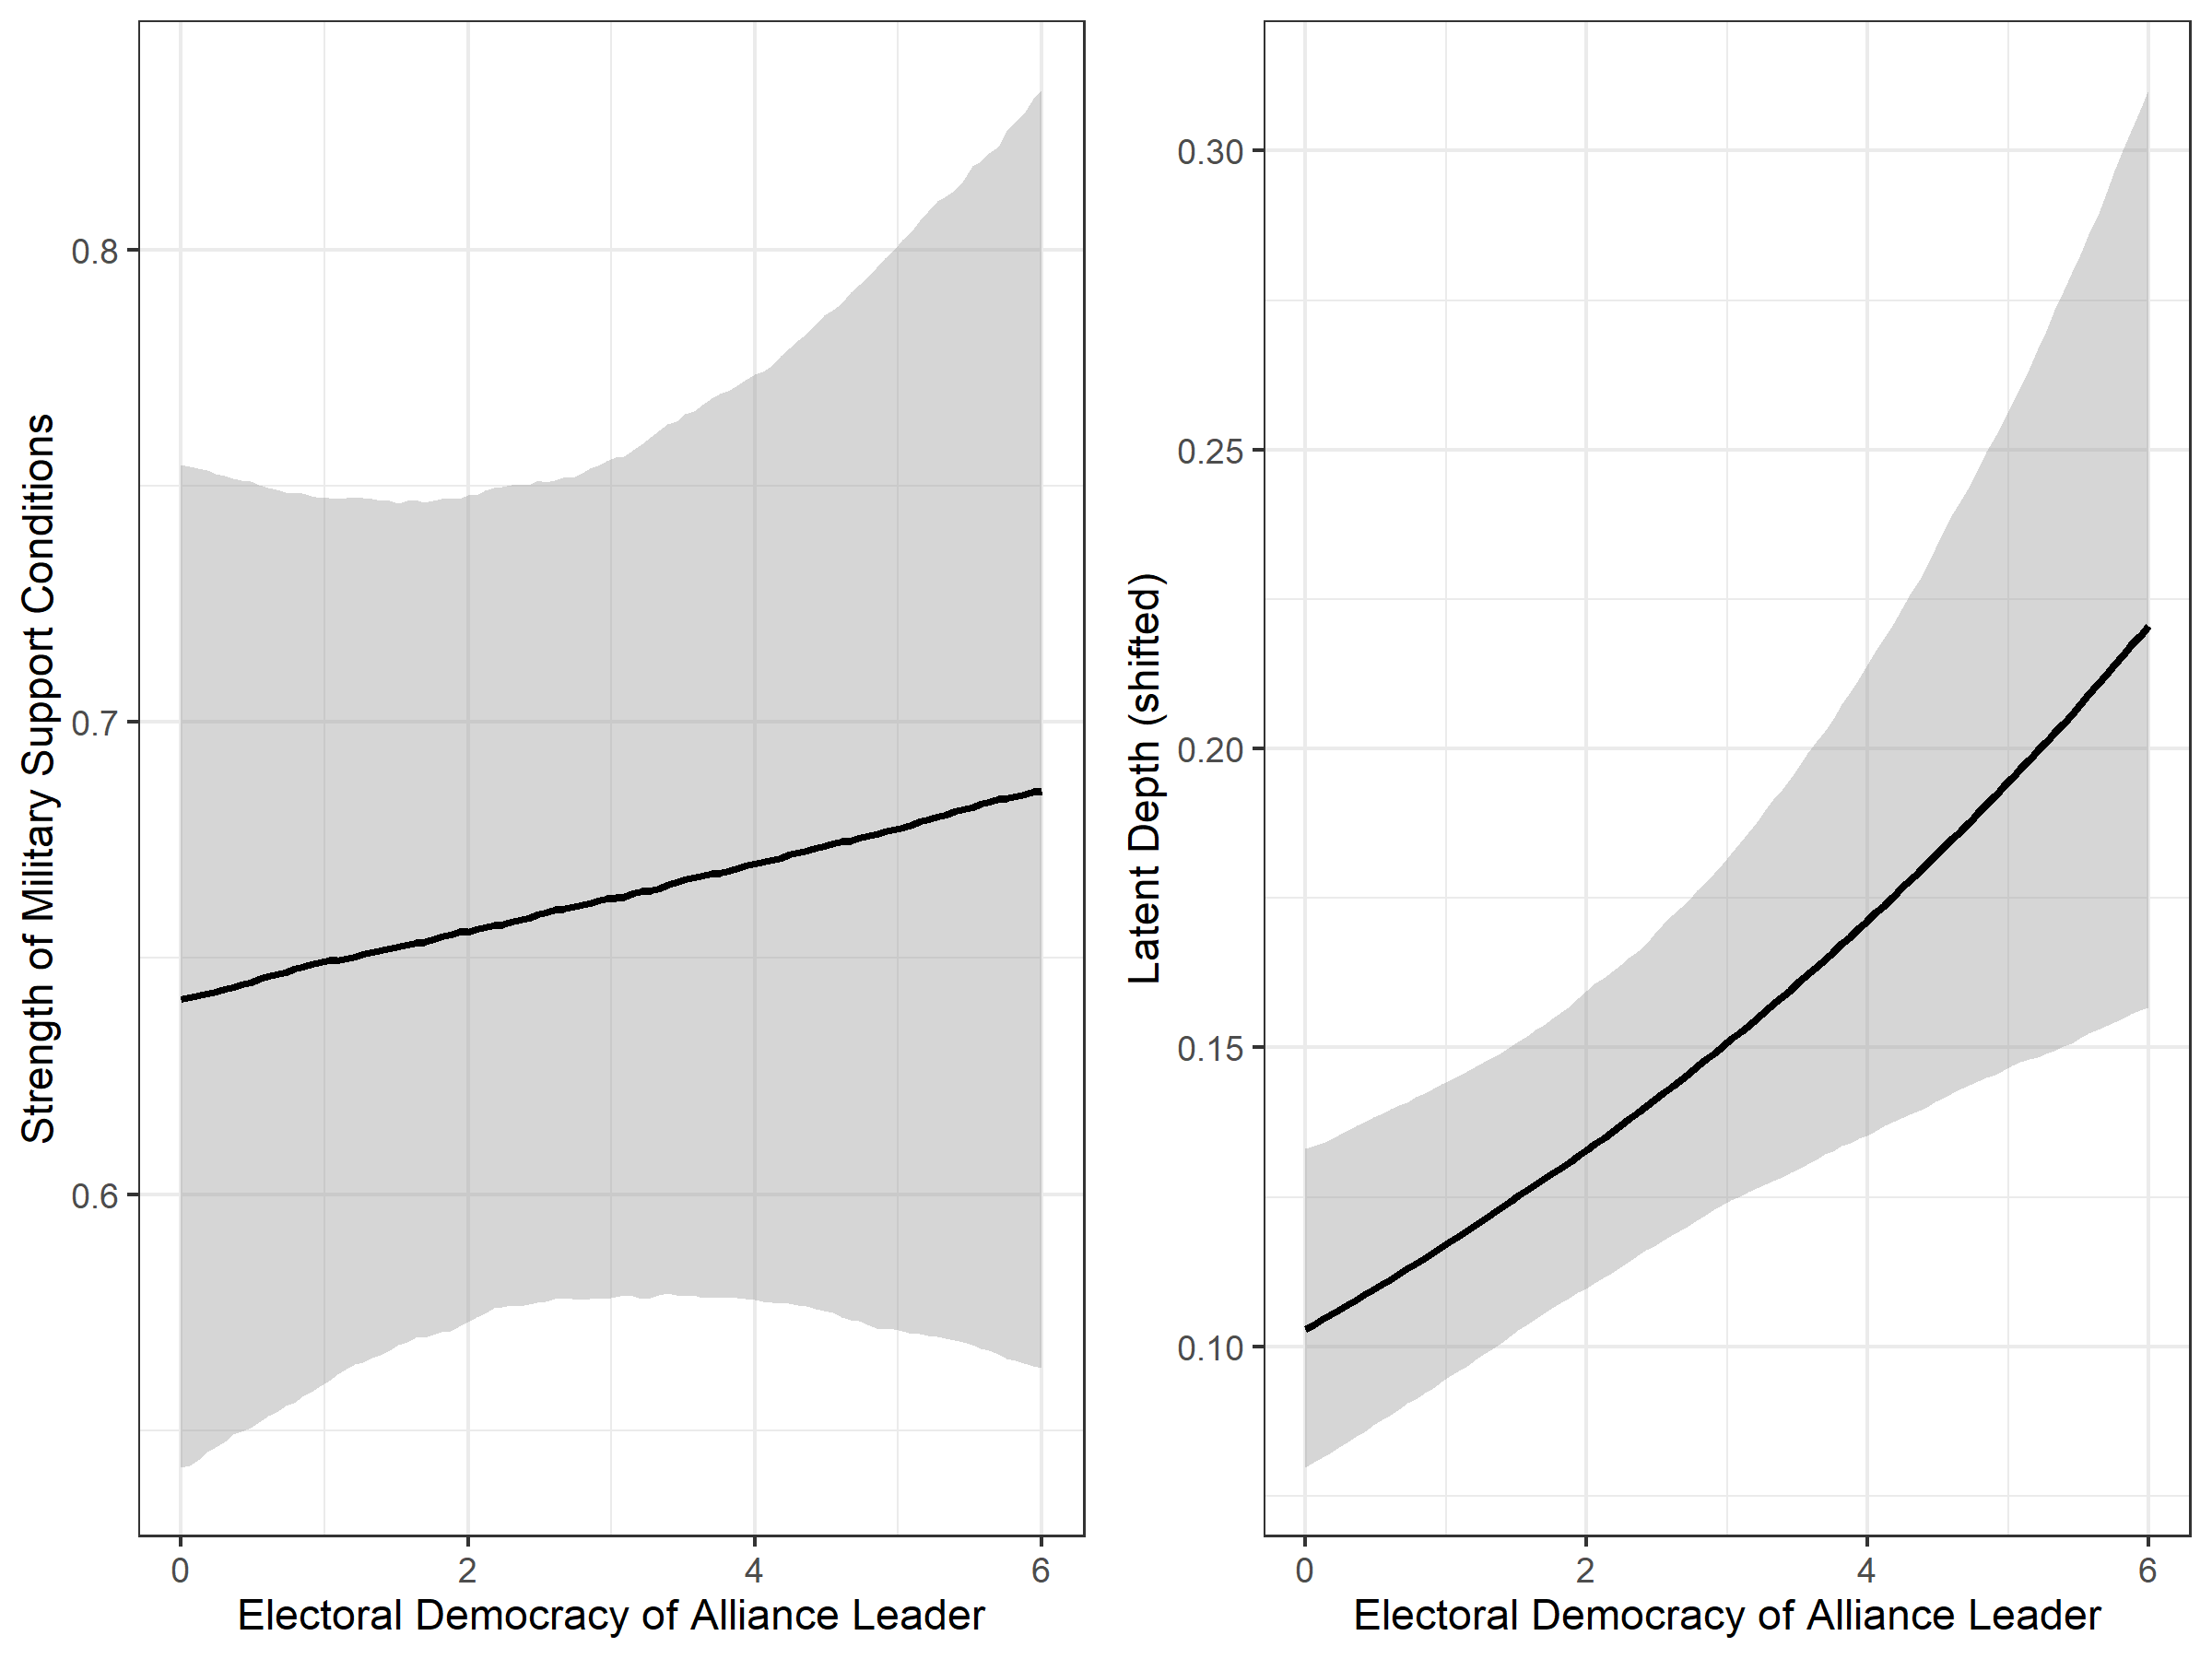
\includegraphics[width=.95\textwidth]{results-joint-hurdle.png}  
\caption{Predicted strength and predicted changes in treaty depth by the the average Polity score of alliance members when the treaty formed based on a joint hurdle model of alliances. The line marks predicted values, and the shaded areas encapsulate the 90\% credible interval. The rug plot on the x-axis marks observed values of allied democracy. Predictions holding all other variables constant.}
\label{fig:results-joint-hurdle}
\end{figure}




\section{Uncertainty in Latent Treaty Depth} 


In the final robustness check, I consider how measurement uncertainty shapes inferences about the connection between non-major power alliances and treaty depth. 
The latent measure of treaty depth has some uncertainty. 
This is a reasonable approximation of alliance politics, because alliance treaty depth is not observed with certainty. 
That said, there are perceptible differences in treaty depth, especially once states add substantial depth to the treaty. 


To incorporate uncertainty over treaty depth, I fit a modification of the joint model. 
First, I created 1,000 alliance datasets, one for each draw of the posterior distribution of the latent measure.
All other variables remained the same, but the treaty depth variables are unique to each dataset. 
Then I fit the model of mean treaty depth to 500 randomly sampled datasets from those 1,000 to facilitate computation. 
For models of depth with uncertainty, I use BRMS \citep{Buerkner2017}. 
Joint Bayesian estimation has the flexibility to incorporate the probit and beta models and can be easily extended to account for uncertainty in the depth measure, but it does not allow correlated errors. 
Fitting the model sequentially to each dataset produces 500 separate models, which I combine into a single model by aggregating the posterior draws into a unified posterior that accounts for uncertainty in the treaty depth measure.\footnote{Standard convergence diagnostics indicate convergence in all 500 models. Diagnostics like $\hat{r}$ are less useful for the full posterior, because some of the chains in the submodels do not overlap.}
This approach is analogous to common techniques for analyzing missing data, where multiple imputation generates uncertainty about the missing values \citep{Hollenbachetal2018imp}.
After multiple imputation, researchers fit a separate model to each imputed dataset and then combine the results. 


% Expand on these results later 
After accounting for uncertainty over treaty depth, I find a similar pattern, but the estimates have more uncertainty. 
I plot the relevant posterior distributions in \autoref{fig:results-unc-depth}. 
The 90\% credible interval for treaty depth barely overlaps zero, but most of the posterior mass is positive. 
Similarly, the 90\% credible interval for the association between alliance leader Polity and unconditional support is largely negative, but it also includes zero and some large positive values. 
In general, there is more uncertainty in the unconditional support estimate. 


\begin{figure}
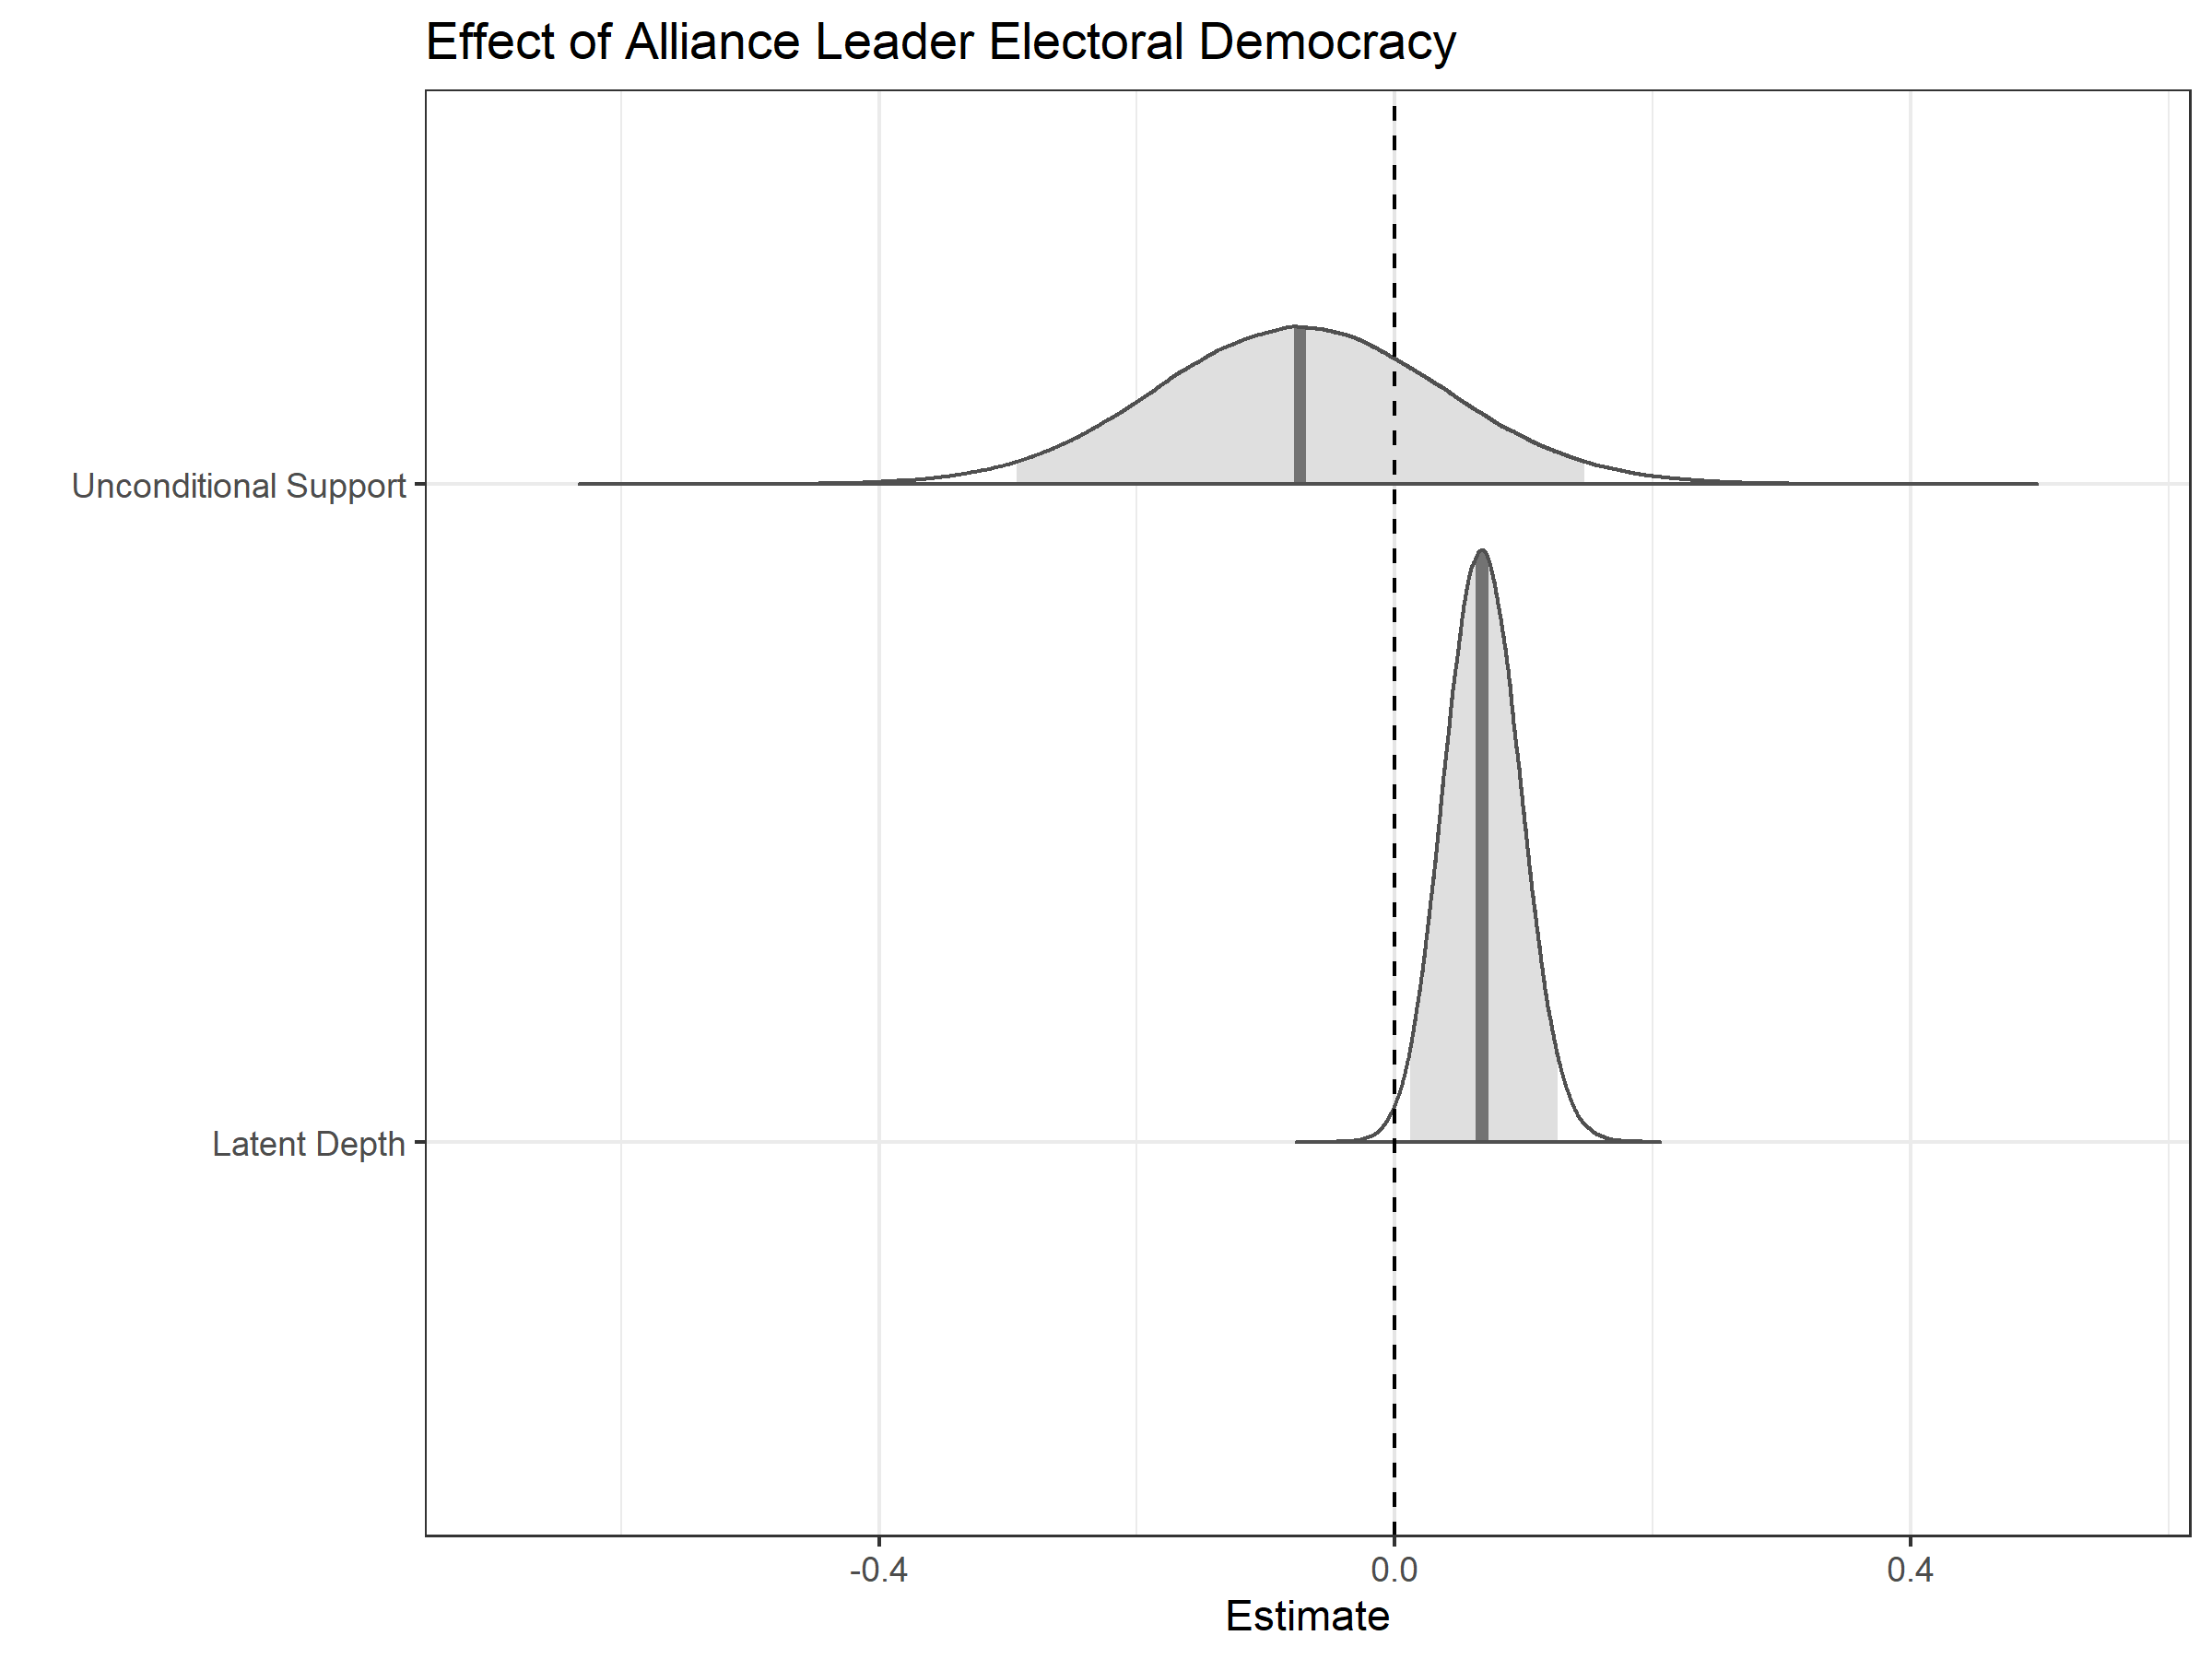
\includegraphics[width=.95\textwidth]{results-unc-depth.png}  
\caption{Estimated association between the democracy of the most capable alliance member and two sources of treaty depth from a Bayesian model that accounts for uncertainty in the latent depth measure. The density plot shows the posterior distributions, and the shaded area summarizes the 90\% credible interval.}
\label{fig:results-unc-depth}
\end{figure}


\section{Issue Linkages and Treaty Credibility}


\citep{Poast2013} observes that issue linkages increase alliance credibility in buffer states.
Because buffer states face high overall threat and generating a credible commitment is difficult, Poast concludes that issue linkages are generally a source of credibility.
In the manuscript, I use issue linkages as a control variable and do not discuss this source of credibility in the theory. 
I offer this minimal discussion of issue linkages to simplify the argument and empirical evidence. 
Examining treaty depth, unconditional military support and issue linkages together is a logical next step in theory development. 


This section of the appendix shows that I make similar inferences about democracy and treaty design in a trivariate model of depth, unconditional military support, and issue linkages. 
All three outcome measures are dummy variables. 
The depth dummy is equal to one if an alliance has greater than the median value of latent treaty depth. 
Unconditional military support is equal to one if the alliance places no conditions on military intervention. 
Last, I set the issue linkages dummy equal to one if the alliance promises economic cooperation. 
I use a joint generalized regression model for estimation. 
The trivariate model converges to the same estimates regardless of the copula, so the results below should be interpreted with some caution.


Even after accounting for correlated errors between models of treaty depth, unconditional military support and issue linkages, I find a positive relationship between the Polity score of the most capable alliance member and treaty depth. 
I also find no clear association between the political institutions of the alliance leader and the probability of unconditional military support. 
\autoref{fig:pred-trivar} summarizes the estimates as predicted probabilities for each possible value of the alliance leaders' Polity score. 
Estimates hold all covariates besides the Polity score of the most capable alliance member at their mode or median.  


\begin{figure}
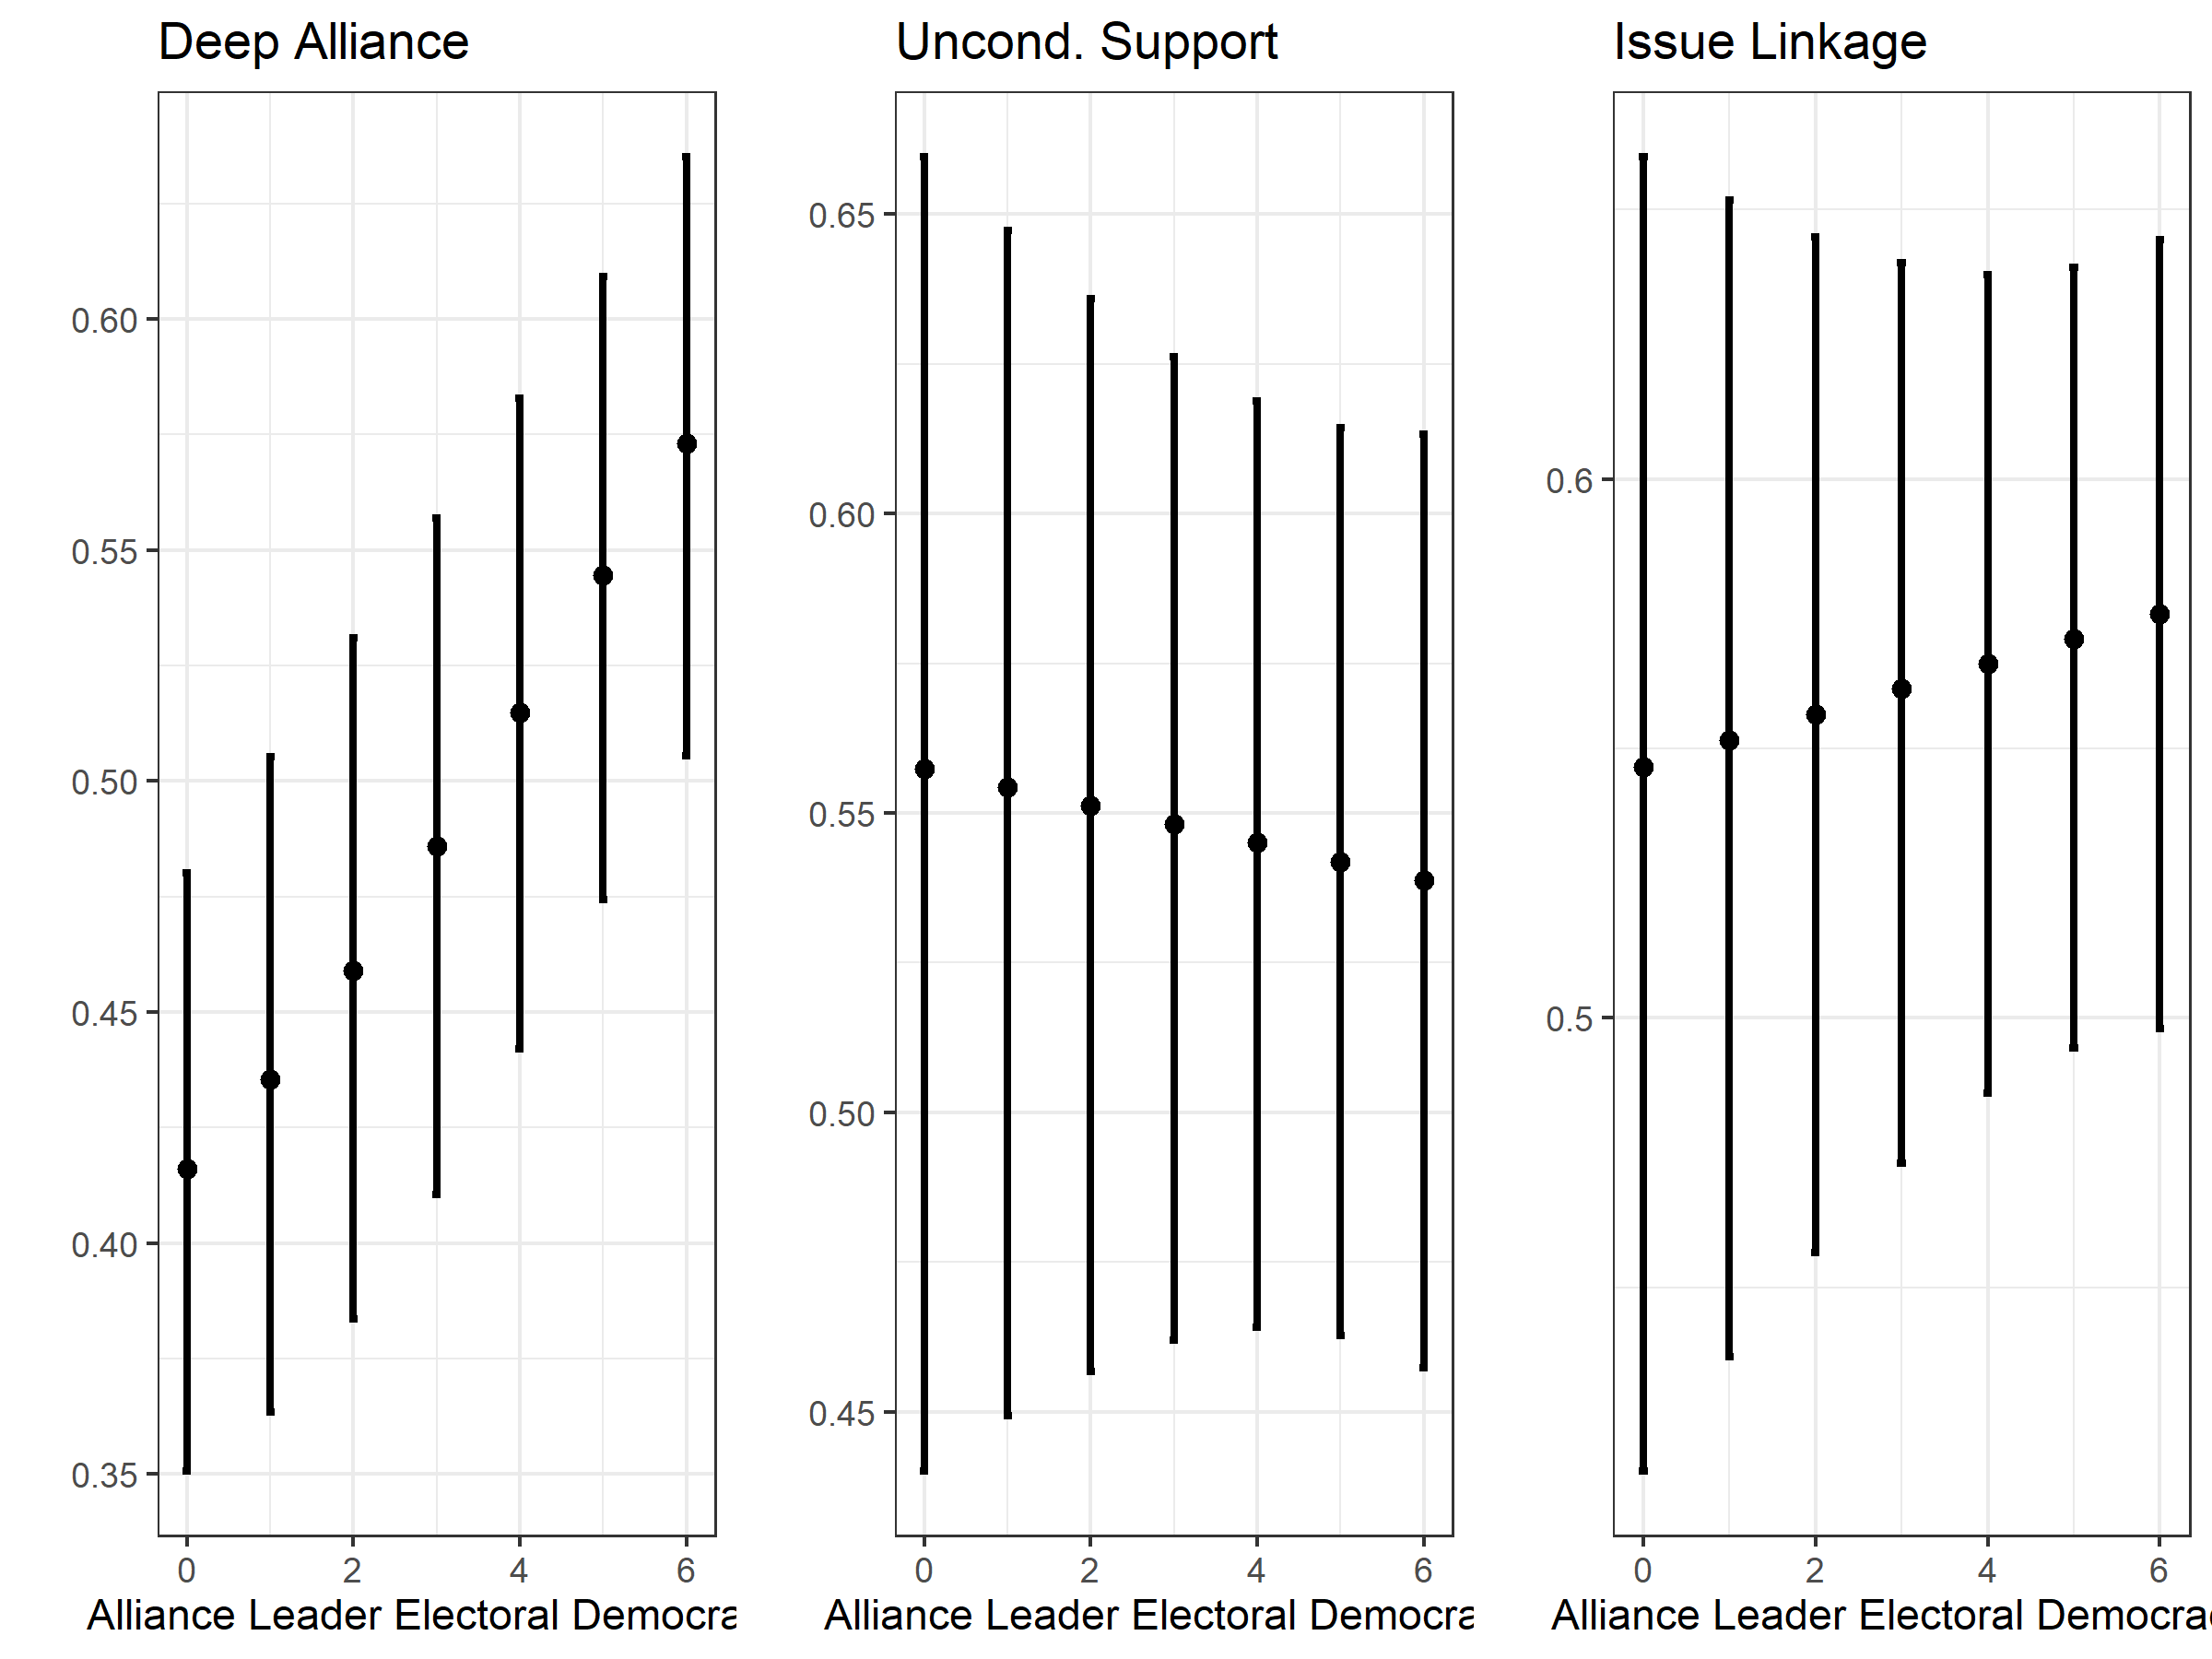
\includegraphics[width=.95\textwidth]{pred-trivar.png}  
\caption{Predicted probabilities an alliance includes three sources of credibility across the range of alliance leader Polity scores. The three outcomes are dummy variables for a deep alliance, unconditional military support, and issue linkages. Predictions based on estimates from a trivariate GJRM model with a normal copula.}
\label{fig:pred-trivar}
\end{figure}




\newpage

\singlespace
 
\bibliography{../../../MasterBibliography} 





\end{document}